% This must be in the first 5 lines to tell arXiv to use pdfLaTeX, which is strongly recommended.

% In particular, the hyperref package requires pdfLaTeX in order to break URLs across lines.

\documentclass[11pt]{article}



% Remove the "review" option to generate the final version.
\usepackage{ACL2023}

% Standard package includes
\usepackage{times}
\usepackage{latexsym}

\usepackage{multirow}

\usepackage{colortbl}

% \usepackage{fontspec}
% \setmainfont{Times New Roman}
% \newfontface{\bn}{kalpurush.ttf}


\usepackage{arydshln}
\usepackage{graphicx}
\usepackage{booktabs}
\usepackage{subcaption}
\usepackage{multirow}
\usepackage{rotating}
\usepackage{amsmath}
\usepackage[normalem]{ulem}
\usepackage{lscape}
\usepackage{ctable}
\usepackage{quoting}
\usepackage{parallel}
\usepackage{graphicx}
\usepackage{ifthen}
\usepackage{tikz}
\usetikzlibrary{calc}
\usepackage[belowskip=-10pt,skip=0.333\baselineskip]{caption}
% \usetikzlibrary{matrix,calc}
% \usepackage{caption}
% \captionsetup[figure]{font={stretch=1.2}}
% For proper rendering and hyphenation of words containing Latin characters (including in bib files)
\usepackage[T1]{fontenc}
\usepackage{array}
\newcolumntype{C}[1]{>{\centering\let\newline\\\arraybackslash\hspace{0pt}}m{#1}}
\newcolumntype{P}[1]{>{\centering\arraybackslash}p{#1}}
% \Xhline{2\arrayrulewidth}

\usepackage{makecell}
\renewcommand\cellalign{lc}
\setcellgapes{3pt}
\makegapedcells
\newcommand\thickvrule[1][0.8pt]{\vrule width #1}
% \usepackage{graphicx}
% \usepackage{ifthen}
% \usetikzlibrary{matrix,calc}
\usepackage{hhline}

% \font \bangla = "Kalpurush:script=beng"
% \newfontfamily\bn{kalpurush.ttf}


% For Vietnamese characters
% \usepackage[T5]{fontenc}
% See https://www.latex-project.org/help/documentation/encguide.pdf for other character sets

% This assumes your files are encoded as UTF8
\usepackage[utf8]{inputenc}

% This is not strictly necessary, and may be commented out.
% However, it will improve the layout of the manuscript,
% and will typically save some space.
\usepackage{microtype}
\usepackage{hyperref}
 
% This is also not strictly necessary, and may be commented out.
% However, it will improve the aesthetics of text in
% the typewriter font.
\usepackage{inconsolata}
\usepackage{tikz}
\usetikzlibrary{arrows}
\usetikzlibrary{backgrounds}
\setlength\doublerulesep{0.5pt} 
% \usepackage[usenames,dvipsnames]{xcolor}

% If the title and author information does not fit in the area allocated, uncomment the following
%
%\setlength\titlebox{<dim>}
%
% and set <dim> to something 5cm or larger.




\title{\textsc{BanglaBook}: A Large-scale Bangla Dataset for Sentiment Analysis from Book Reviews} % Reviews (?)

% Author information can be set in various styles:
% For several authors from the same institution:
% \author{Author 1 \and ... \and Author n \\
%         Address line \\ ... \\ Address line}
% if the names do not fit well on one line use
%         Author 1 \\ {\bf Author 2} \\ ... \\ {\bf Author n} \\
% For authors from different institutions:
% \author{Author 1 \\ Address line \\  ... \\ Address line
%         \And  ... \And
%         Author n \\ Address line \\ ... \\ Address line}
% To start a seperate ``row'' of authors use \AND, as in
% \author{Author 1 \\ Address line \\  ... \\ Address line
%         \AND
%         Author 2 \\ Address line \\ ... \\ Address line \And
%         Author 3 \\ Address line \\ ... \\ Address line}

% \author{First Author \\
%   Affiliation / Address line 1 \\
%   Affiliation / Address line 2 \\
%   Affiliation / Address line 3 \\
%   \texttt{email@domain} \\\And
%   Second Author \\
%   Affiliation / Address line 1 \\
%   Affiliation / Address line 2 \\
%   Affiliation / Address line 3 \\
%   \texttt{email@domain} \\}
%%%%%%%
% TODO:
% - add Github footnote (in abstract and final table)
% - other contributions in itemize block (done)
% - tSNE plot (?)
% - color coding significance in the caption of table (done)
% - train-dev-test split of the dataset (done)
% - Mixed vs Bangla + English maneh ki caption eh likha (done)
% - Remove template's appendix
%%%%%%%

\author{\bf Mohsinul Kabir$^*$, 
{\bf Obayed Bin Mahfuz$^*$,}
{\bf Syed Rifat Raiyan$^*$,}\\ 
{\bf Hasan Mahmud,}
{\bf Md Kamrul Hasan}\\
Systems and Software Lab (SSL)\\ Department of Computer Science and Engineering\\
Islamic University of Technology, Dhaka, Bangladesh\\
\texttt{\{mohsinulkabir, siam, rifatraiyan, hasan, hasank\}@iut-dhaka.edu}\\
}

\begin{document}
\font \bangla = "Kalpurush:script=beng"
\font \smallbangla = "Kalpurush:script=beng" at 9pt

\maketitle
\def\thefootnote{*}\footnotetext{These authors contributed equally to this work. Author names are in alphabetic order. }
\def\thefootnote{\arabic{footnote}}
\begin{abstract}
The analysis of consumer sentiment, as expressed through reviews, can provide a wealth of insight regarding the quality of a product. While the study of sentiment analysis has been widely explored in many popular languages, relatively less attention has been given to the Bangla language, mostly due to a lack of relevant data and cross-domain adaptability. To address this limitation, we present \textsc{BanglaBook}, a large-scale dataset of Bangla book reviews consisting of 158,065 samples classified into three broad categories: positive, negative, and neutral. We provide a detailed statistical analysis of the dataset and employ a range of machine learning models to establish baselines including SVM, LSTM, and Bangla-BERT. Our findings demonstrate a substantial performance advantage of pre-trained models over models that rely on manually crafted features, emphasizing the necessity for additional training resources in this domain. Additionally, we conduct an in-depth error analysis by examining sentiment unigrams, which may provide insight into common classification errors in under-resourced languages like Bangla. Our codes and data are publicly available at \url{https://github.com/mohsinulkabir14/BanglaBook}.
\end{abstract}

\section{Introduction}
%Sentiment analysis (SA) is defined as the computational study of mining individuals' subjective opinions, emotions, and appraisals towards products and services. A significant amount of research on SA in a variety of languages, including English, Arabic, Chinese, and French, has been conducted across a wide range of domains \citep{bhowmik2021bangla}. In contrast, 
The resources publicly available for scholarly investigation in the realm of Sentiment Analysis (SA) for the Bangla language are scarce and limited in quantity \citep{khatun2022machine, sazzed2021bengsentilex, rahman2019annotated} despite its literary gravitas as the 6\textsuperscript{th} most spoken language\footnote{\url{https://en.wikipedia.org/wiki/List_of_languages_by_total_number_of_speakers}} in the world with approximately 200 million speakers.
%\\
%A major drawback of the existing literature on Bangla Text SA is the scarcity of publicly available datasets. 
In the existing literature on Bangla Text SA, as shown in Table \ref{tab:dataset_comparison}, the largest dataset consists of 20,468 samples \citep{islam2022emonoba} while the smallest has a mere 1,050 samples \citep{tabassum2019design}. Besides these, \citet{islam2020sentiment} created a dataset consisting of 17,852 samples and \citet{islam2021sentnob} utilized a dataset of 15,728 samples. All other datasets apart from these either have $<$15,000 samples or are publicly unavailable.\\
Another limitation of the existing research works in Bangla Text SA is the deficiency of datasets having product-specific review samples. Most of the available Bangla SA datasets are focused on user-generated textual content from cyberspace. The insights derived from these may not accurately represent sentiment in the context of product reviews, thus hindering their usefulness for businesses. The tonal and linguistic analysis of reviews from product-specific datasets can aid businesses to gain valuable insights into customer attitudes, preferences, and experiences which can then be leveraged to improve products and services, design targeted marketing campaigns, and make more informed business decisions. In this paper, we introduce a large-scale dataset, \textsc{BanglaBook}, consisting of 158,065 samples of book reviews collected from online bookshops written in the Bangla language. This is the largest dataset for Bangla sentiment analysis to the best of our knowledge. We perform an analysis of the dataset's statistical characteristics, employ various ML techniques to establish a performance benchmark for validating the dataset, and also conduct a thorough evaluation of the classification errors.
% In this paper, our contributions are,
% \begin{itemize}
%     \item We introduce a large-scale dataset, \textsc{BanglaBook}, consisting of 1,58,065 samples of book reviews collected from online bookshops written in the Bangla language.
% \end{itemize}
\begin{table*}[ht]
\centering
\setlength\doublerulesep{0.65pt}
\scriptsize
\begin{tabular}{c|c|c|c|c}
\hline
\textbf{Source}       & \textbf{Language}        & \textbf{Annotated} & \textbf{Unannotated} & \textbf{Total} \\ \hline
                      & Bangla                   & 84,672             & 24,806               & 109,478        \\
Rokomari              & Bangla\textsuperscript{\textdagger} + English         & 56,485             & 15,408               & 71,893         \\
                      & Bangla + Bangla\textsuperscript{\textdagger} + English                    & 13,144             & 4,114                & 17,258         \\ \cline{2-5} 
                      & Total                    & 154,301            & 44,328               & 198,629        \\ \hline
                      & Bangla                   & 4,699              & 59                   & 4,758          \\
Wafilife             & Bangla\textsuperscript{\textdagger} + English         & 370                & 3                    & 373            \\
                      & Bangla + Bangla\textsuperscript{\textdagger} + English                    & 896                & 3                    & 899            \\ \cline{2-5} 
                      & Total                    & 5,965              & 65                   & 6,030          \\ \hline
                      & Bangla                   & 89,371             & 24,865               & 114,237        \\
                      & Bangla\textsuperscript{\textdagger} + English         & 56,855             & 15,411               & 72,266         \\
                      & Bangla + Bangla\textsuperscript{\textdagger} + English                    & 14,040             & 4,117                & 18,157         \\ \cline{2-5}  
                      & Total                    & 160,266            & 44,393               & 204,659        \\ \hline
                      & Untranslated Data (Removed)                                      & 2,201                                   &                                           &                \\ \Xcline{1-5}{0.8pt}
                      & Final Dataset Size                                      & \textbf{158,065}                                   &                                           &                \\ \hline
\end{tabular}
\caption{Summary statistics of our dataset. Bangla\textsuperscript{\textdagger} denotes Romanized Bangla text.}
\label{tab:tab1}
\end{table*}

\section{Dataset Construction}

In order to create this dataset, we collect a total of 204,659 book reviews from two online bookshops (Rokomari\footnote{\url{https://www.rokomari.com/}} and Wafilife\footnote{\url{https://www.wafilife.com/}}) using a web scraper developed with several Python libraries, including \verb|BeautifulSoup|, \verb|Selenium|, \verb|Pandas|, \verb|Openpyxl|, and \verb|Webdriver|, to collect and process the raw data.

% The data collection and preparation process that we follow for this dataset is a five-step process. First, we gather a list of URLs for books available on the aforementioned online bookshops. Next, we collect information about the books, including the names of the books and their authors, as well as the names of the categories they belong to and lists of reviews. In the third step, we collect the text of the reviews, along with ratings, reviewer names, and review dates. In the fourth step, we translate any English, Banglish (written with a combination of English and Bangla), or Romanized Bangla text into Bangla. Finally, in the fifth step, we label each review as positive, negative, or neutral based on ratings ranging from 1 to 5.
For the data collection and preparation process of the \textsc{BanglaBook} dataset, we first compile a list of URLs for authors from online bookstores. From there, we procure URLs for the books. We meticulously scrape information such as book titles, author names, book categories, review texts, reviewer names, review dates, and ratings by utilizing these book URLs. 
% We translate the review texts to Bangla and appropriately label them as positive, negative, or neutral.


\begin{table}[h]
 \centering
 \small
 \begin{tabular}{cc|c}
 \hline
 \parbox[t]{2mm}{\multirow{3}{*}{\rotatebox[origin=c]{90}{\begin{tabular}{c}\textbf{General} \\ \textbf{Properties}\end{tabular}}}} & \multicolumn{1}{c|}{\quad \# of Reviews} & \multicolumn{1}{c}{158,065}\\
 & \multicolumn{1}{c|}{\quad \# of Books} & \multicolumn{1}{c}{30,253}\\
 & \multicolumn{1}{c|}{\quad \# of Reviewers} & \multicolumn{1}{c}{44,616}\\
 & \multicolumn{1}{c|}{\quad \# of Categories} & \multicolumn{1}{c}{1,573}\\
 & \multicolumn{1}{c|}{\quad Total Review Words} & \multicolumn{1}{c}{44,429,201}\\
 \hline
 \parbox[t]{2mm}{\multirow{3}{*}{\rotatebox[origin=c]{90}{\begin{tabular}{@{}c@{}}\textbf{Single}\\ \textbf{Review}\end{tabular}}}} & \multicolumn{1}{c|}{\quad max. Word length} & \multicolumn{1}{c}{765}\\
 & \multicolumn{1}{c|}{\quad min. Word length} & \multicolumn{1}{c}{1}\\
 & \multicolumn{1}{c|}{\quad avg. Word length} & \multicolumn{1}{c}{281.08}\\
 \hline
 \end{tabular}
 \caption{General overview of \textsc{BanglaBook}.}
 \label{tab:tab2}
 \end{table}

 % \vspace{-10pt}



 
\subsection{Labeling \& Translation}
% If a review lacks a rating, it is deemed to be unannotated. 
If a review does not have a rating, we deem it unannotated. Reviews with a rating of 1 or 2 are classified as negative, a rating of 3 is considered neutral, and a rating of 4 or 5 is classified as positive. Two manual experiments are carried out to validate the use of ratings as a measure of sentiment in product reviews. In the first experiment, around 10\% of the reviews are randomly selected and annotated manually. The annotated labels are cross-checked with the original labels, resulting in a 96.7\% accuracy in the corresponding labels. In addition, we consult the work of \citet{Wang2020ARC} that explored the issue of incongruous sentiment expressions with regard to ratings. Specifically, the study scrutinized two categories of reviews: \textit{high ratings lacking a positive sentiment}, and \textit{low ratings lacking a negative sentiment}. We perform an analysis to identify such inconsistencies within our dataset and discovered that only a minuscule 3.41\% of the samples exhibited this pattern. This figure is relatively insignificant when considering the substantially large scale of our dataset.
 %%%%%%%%%%%%%%%%%%%%%%%%%%%%%%%%%%%%%%%%%%%%%%
\begin{figure}[h]
    \centering
    \subfloat[Sentiment Distribution\label{fig:donut_charta}]{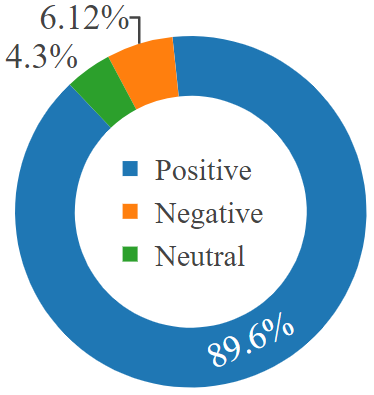
\includegraphics[scale=0.427]{images/ACLBookReview4.PNG}}\hspace{0.05cm}\subfloat[Rating Distribution\label{fig:donut_chartb}]{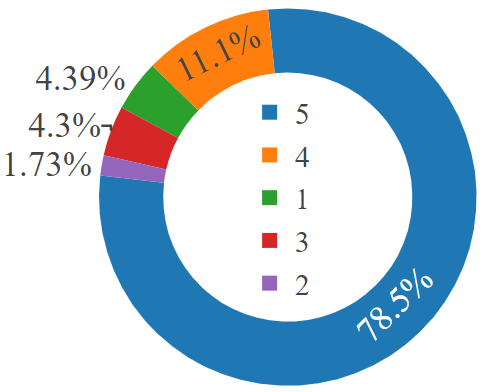
\includegraphics[scale=0.4]{images/ACLBookReview5.PNG}}
    % 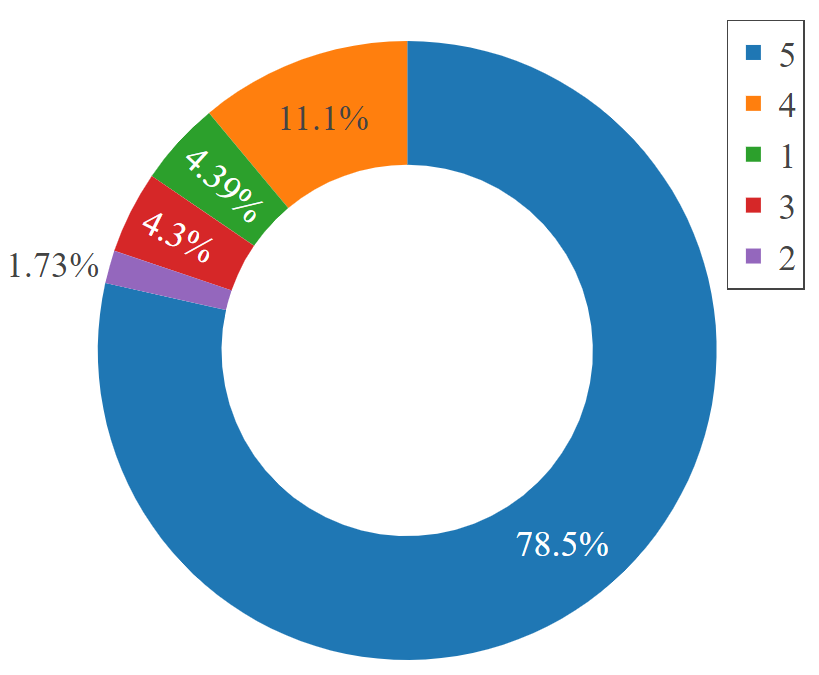
\includegraphics[scale=0.35]{images/ACLBookReview1.PNG}
    \vspace{10pt}
    \caption{Class Distribution of \textsc{BanglaBook}.}
    \label{fig:donut_chart}
\end{figure}
\\
%%%%%%%%%%%%%%%%%%%%%%%%%%%%%%%%%%%%%%%%%%%%%%
After discarding the unannotated reviews, we curate a final dataset of 158,065 annotated reviews. Of these, 89,371 are written entirely in Bangla. The remaining 68,694 reviews were written in Romanized Bangla, English, or a mix of languages. They are translated into Bangla with Google Translator and a custom Python program using the \verb|googletrans| library. The translations are subsequently subjected to manual review and scrutiny to confirm their accuracy. The majority of inaccurate translations primarily comprise spelling errors and instances where English words remain untranslated within samples containing a combination of Bangla and English text. The meticulous evaluation process of untranslated samples involves a thorough assessment by post-graduate native Bangla speakers, who critically compare the translated text against the original untranslated text to ascertain the correctness of the translation.
%%%%%%%%%%%%%%%%%%%%%%%%%%%%%%%%%%%%%%%%%%%%%%%%%%%%
\begin{table*}[htbp]
\centering
\scriptsize
 \begin{tabular}{p{8.0cm} P{1.1cm} P{1.1cm} P{1.1cm} P{2.0cm}} 
\toprule \textbf{Method} & \textbf{Negative}  & \textbf{Neutral}  & \textbf{Positive}  & \textbf{Weighted Avg.}  \\ \midrule
Random Forest{\fontfamily{qcr}\selectfont (word 2-gram + word 3-gram)} & 0.56 & 0.34 & 0.96 & 0.9106\\
SVM{\fontfamily{qcr}\selectfont (word 2-gram + word 3-gram)} & 0.40 & 0.15 & \textbf{1.00} & 0.9053\\
Random Forest{\fontfamily{qcr}\selectfont (word 1-gram)} & 0.48 & 0.35 & 0.96 & 0.9043\\
Logistic Regression{\fontfamily{qcr}\selectfont (char 2-gram + char 3-gram)} & 0.55 & 0.13 & 0.96 & 0.8978\\
Bangla-BERT{\fontfamily{qcr}\selectfont(base-uncased)} & 0.60 & 0.22 & 0.96 & 0.9064\\
Logistic Regression{\fontfamily{qcr}\selectfont (word 2-gram + word 3-gram)} & 0.53 & 0.13 & 0.96 & 0.8964\\
Bangla-BERT{\fontfamily{qcr}\selectfont (large)} & \textbf{0.72} & \textbf{0.40} & 0.97 & \textbf{0.9331}\\
\hdashline 
XGBoost{\fontfamily{qcr}\selectfont (char 2-gram + char 3-gram)} & 0.31 & 0.02 & 0.95 & 0.8723\\
Multinomial NB{\fontfamily{qcr}\selectfont (word 2-gram + word 3-gram)} & 0.23 & 0.03 & 0.95 & 0.8663\\
LSTM{\fontfamily{qcr}\selectfont (GloVe)} & 0.11 & 0.00 & 0.10 & 0.0991\\
XGBoost{\fontfamily{qcr}\selectfont (word 2-gram + word 3-gram)} & 0.23 & 0.01 & 0.95 & 0.8651\\
Multinomial NB{\fontfamily{qcr}\selectfont (BoW)} & 0.18 & 0.05 & 0.94 & 0.8564\\
SVM{\fontfamily{qcr}\selectfont (word 1-gram)} & 0.08 & 0.04 & 0.94 & 0.8519\\

\bottomrule
\end{tabular}
\caption{Catergory-wise Binary Task F1-score and Weighted Average F1-score of each method on \textsc{BanglaBook}.}\label{tab:baseline}
% \vspace{-10pt}
\end{table*}
%%%%%%%%%%%%%%%%%%%%%%%%%%%%%%%%%%%%%%%%%%%%%%%%%%%




%The translations are then manually inspected to ensure accuracy.


\section{Statistical Analysis}
Tables \ref{tab:tab1} and \ref{tab:tab2} provide an overview of the statistical properties of the \textsc{BanglaBook} dataset. The sentiment doughnut chart in Figure-\ref{fig:donut_charta} illustrates the proportion of positive, neutral, and negative reviews, while the rating doughnut chart in Figure-\ref{fig:donut_chartb} displays the percentage of reviews that correspond to each rating on a scale of 1 to 5.

\definecolor{NavyBlue}{HTML}{0066CC}
\definecolor{ForestGreen}{HTML}{228B22}
\definecolor{Lavender}{HTML}{745BB1}
\definecolor{Crimson}{HTML}{DC143C}
\definecolor{Red}{HTML}{FF0000}
\definecolor{Cyan}{HTML}{33FFFF}
\definecolor{LightGreen}{HTML}{80FF00}
\definecolor{Gold}{HTML}{CCCC00}
\definecolor{Pink}{HTML}{FF00FF}
Upon analyzing the sentiment chart, it appears that the majority of the reviews (\textcolor{NavyBlue}{124,084} + \textcolor{orange}{17,503} = 141,587 samples) are positive, with a significant portion also being negative (\textcolor{Lavender}{2,728} + \textcolor{ForestGreen}{6,946} = 9,674 samples). A relatively small fraction of the reviews are neutral (\textcolor{Crimson}{6,804} samples). This suggests that overall, the books have been well received by the readers, with the majority expressing favorable opinions. The distribution of the dataset is representative of real-world scenarios and it tessellates well with previous content analysis works on book reviews \cite{lin2005effect,sorensen2004any}. 
% In the rating chart, it is evident that the majority of the reviews have awarded the books a high rating, with a large number of 5-star (1,24,084 samples) and 4-star reviews (17,503 samples). There is a relatively small number of 1-star (6,946 samples) and 2-star (2,728 samples) reviews, indicating that the books have received mostly positive ratings.
In Figure-\ref{fig:categorywise}, we can visualize an illustration of the sentiment distribution among the 5 most frequently reviewed categories of books. We can gain some salient insights from the popularity of these genres. Contemporary novels are bestsellers as they reflect current events, social issues, and trends, making them relatable and thought-provoking for the readers while self-help and religious books provide guidance, inspiration, and a sense of purpose, catering to individuals' quest for personal growth and spiritual fulfillment.

\begin{figure}[h]
    \centering
    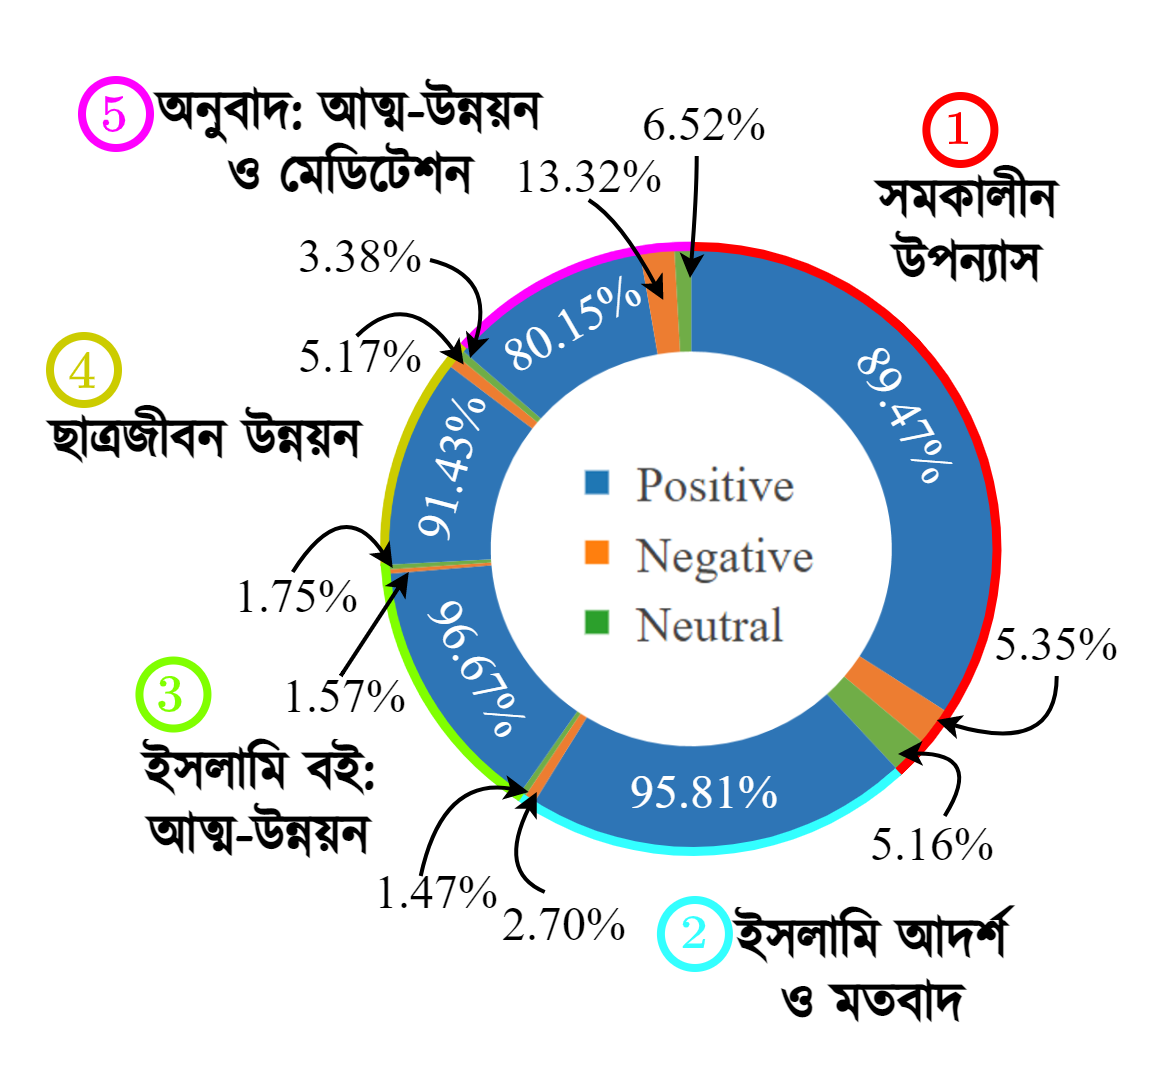
\includegraphics[scale=0.19]{images/ACLBookReview8.PNG}
    \caption{$\text{Sentiment}\hspace{2.5pt}\text{Distribution}\hspace{2.5pt}\text{of}\hspace{2.5pt}\text{top}\hspace{2.5pt}\text{5}\hspace{2.5pt}\text{most}\hspace{2.5pt}\text{popular}$$\\$genres.$\hspace{2.5pt}$In$\hspace{2.5pt}$clockwise$\hspace{2.5pt}$order,$\hspace{2.5pt}$\bangla  \textcolor{Red}{সমকালীন}$\hspace{2pt}$\textcolor{Red}{উপন্যাস}$\hspace{2pt}$$\text{(Contemp-}\\\text{orary}$$\hspace{2.5pt}$$\text{Novel)}$,$\hspace{2pt}$\bangla \textcolor{Cyan}{ইসলামি}$\hspace{2pt}$\textcolor{Cyan}{আদর্শ}$\hspace{2pt}$\textcolor{Cyan}{ও}$\hspace{2pt}$\textcolor{Cyan}{মতবাদ}$\hspace{2pt}$$\text{(Islamic}\hspace{2.5pt}\text{Ideals} \hspace{2.5pt}\text{and}$$\\$$\text{Doctrines),}$$\hspace{2pt}$\bangla \textcolor{LightGreen}{ইসলামি}$\hspace{2.5pt}$\textcolor{LightGreen}{বই:}$\hspace{2.5pt}$\textcolor{LightGreen}{আত্ম}$\hspace{2.5pt}$\textcolor{LightGreen}{উন্নয়ন}$\hspace{2.5pt}$$\text{(Islamic}\hspace{2.5pt}\text{Books:}\hspace{2.5pt}\text{Self-}\\\text{Development)}$,$\hspace{2.5pt}$\bangla \textcolor{Gold}{ছাত্রজীবন}$\hspace{2.5pt}$\textcolor{Gold}{উন্নয়ন}$\hspace{2.5pt}$$\text{(Student}\hspace{2.5pt}\text{Life}\hspace{2.5pt}\text{Developm-}\\\text{ent)}$,$\hspace{2.5pt}$\bangla \textcolor{Pink}{অনুবাদ:}$\hspace{2.5pt}$\textcolor{Pink}{আত্ম-উন্নয়ন}$\hspace{2.5pt}$\textcolor{Pink}{ও}$\hspace{2.5pt}$\textcolor{Pink}{মেডিটেশন}$\hspace{2.5pt}$$\text{(Translated}\hspace{2.5pt}\text{Books:}\\\text{Self-Development}$$\hspace{2pt}$$\text{and}\hspace{2.5pt}\text{Meditation).}$}
    \label{fig:categorywise}
\end{figure}
% \begin{figure}[h]
%     \centering
%     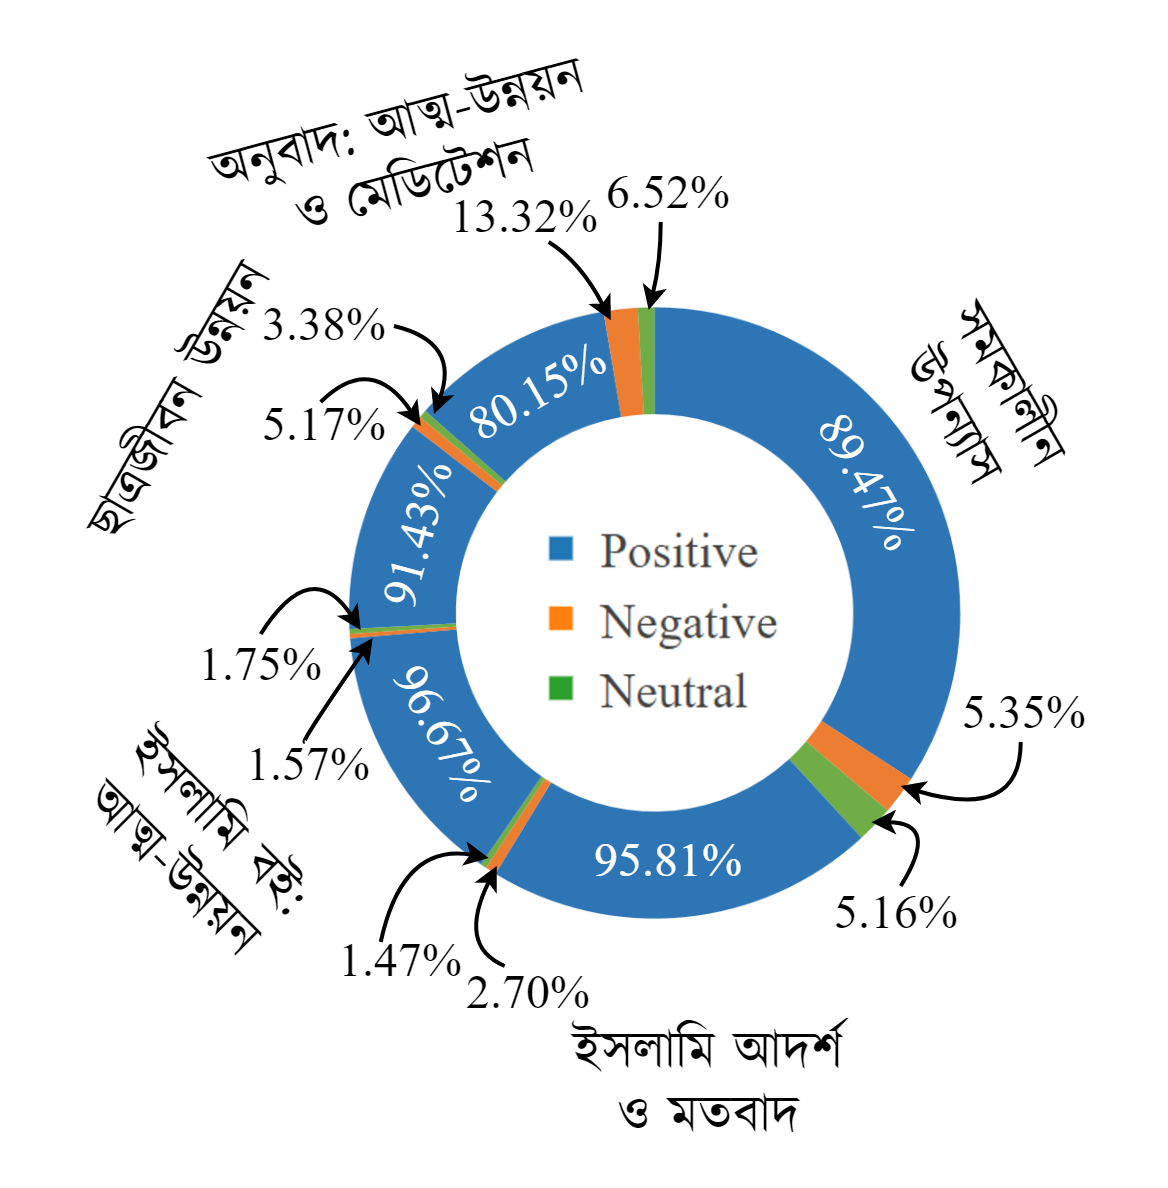
\includegraphics[scale=0.13]{images/ACLBookReview6.PNG}
%     \caption{Sentiment Distribution of top 5 most popular genres. In clockwise order, \bangla সমকালীন উপন্যাস $\text{(Contemporary Novel)}$, \bangla ইসলামি আদর্শ ও মতবাদ $\text{(Islamic Ideals and Doctrines)}$, \bangla ইসলামি বই: আত্ম-উন্নয়ন $\text{(Islamic Books: Self-Development)}$, \bangla ছাত্রজীবন উন্নয়ন $\text{(Student Life Development)}$, \bangla অনুবাদ: আত্ম-উন্নয়ন ও মেডিটেশন $\text{(Translated Books: Self-Development and Meditation)}$}
%     \label{fig:categorywise}
% \end{figure}


\section{Developing Benchmark for \textsc{BanglaBook}}




% \def\myConfMat{{
% {77, 38, 1792},  %row 1
% {52, 21, 1272},  %row 2
% {1222, 424, 26508},  %row 3
% }}

% \def\classNames{{"Negative","Neutral","Positive"}} %class names. Adapt at will

% \def\numClasses{3} %number of classes. Could be automatic, but you can change it for tests.

% \def\myScale{1.5} % 1.5 is a good scale. Values under 1 may need smaller fonts!
% \begin{tikzpicture}[
%     scale = \myScale,
%     %font={\scriptsize}, %for smaller scales, even \tiny may be useful
%     ]
%     \centering

% \tikzset{vertical label/.style={rotate=90,anchor=east}}   % usable styles for below
% \tikzset{diagonal label/.style={rotate=45,anchor=north east}}

% \foreach \y in {1,...,\numClasses} %loop vertical starting on top
% {
%     % Add class name on the left
%     \node [anchor=east] at (0.4,-\y) {\small \rotatebox{90}{\pgfmathparse{\classNames[\y-1]}\pgfmathresult}}; 
    
%     \foreach \x in {1,...,\numClasses}  %loop horizontal starting on left
%     {
% %---- Start of automatic calculation of totSamples for the column ------------   
%     \def\totSamples{0}
%     \foreach \ll in {1,...,\numClasses}
%     {
%         \pgfmathparse{\myConfMat[\ll-1][\x-1]}   %fetch next element
%         \xdef\totSamples{\totSamples+\pgfmathresult} %accumulate it with previous sum
%         %must use \xdef fro global effect otherwise lost in foreach loop!
%     }
%     \pgfmathparse{\totSamples} \xdef\totSamples{\pgfmathresult}  % put the final sum in variable
% %---- End of automatic calculation of totSamples ----------------
    
%     \begin{scope}[shift={(\x,-\y)}]
%         \def\mVal{\myConfMat[\y-1][\x-1]} % The value at index y,x (-1 because of zero indexing)
%         \pgfmathtruncatemacro{\r}{\mVal}   %
%         \pgfmathtruncatemacro{\p}{round(\r/\totSamples*100)}
%         \coordinate (C) at (0,0);
%         \ifthenelse{\p<50}{\def\txtcol{black}}{\def\txtcol{white}} %decide text color for contrast
%         \node[
%             draw,                 %draw lines
%             text=\txtcol,         %text color (automatic for better contrast)
%             align=center,         %align text inside cells (also for wrapping)
%             fill=green!\p,        %intensity of fill (can change base color)
%             minimum size=\myScale*10mm,    %cell size to fit the scale and integer dimensions (in cm)
%             inner sep=0,          %remove all inner gaps to save space in small scales
%             ] (C) {\r};     %text to put in cell (adapt at will)
%         %Now if last vertical class add its label at the bottom
%         \ifthenelse{\y=\numClasses}{
%         \node [] at ($(C)-(0,0.75)$) % can use vertical or diagonal label as option
%         {\small\pgfmathparse{\classNames[\x-1]}\pgfmathresult};}{}
%     \end{scope}
%     }
% }
% %Now add x and y labels on suitable coordinates
% \coordinate (yaxis) at (-0.1,0.2-\numClasses/2);  %must adapt if class labels are wider!
% \coordinate (xaxis) at (0.5+\numClasses/2, -\numClasses-1.0); %id. for non horizontal labels!
% \node [vertical label] at (yaxis) {\textbf{True Labels}};
% \node []               at (xaxis) {\textbf{Predicted Labels}};
% \end{tikzpicture}

%%%%%%%%%%%%%%%%%%%%%%%%%%%%%%%%%%%%%%%%%%%%%
\begin{table*}[h]
\centering
\small
\begin{tabular}{p{1.1 cm}|P{14 cm}}
\hline
\textbf{Class}    & \textbf{10 Most Frequent Words} \\ \hline
\textbf{Positive} &    \colorbox{lime!50}{\bangla ভালো $\text{(good)}$}$\text{,}$ \colorbox{lime!50}{\bangla সুন্দর $\text{(nice)}$}$\text{,}$ \colorbox{lime!50}{\bangla অসাধারণ $\text{(extraordinary)}$}$\text{,}$  \colorbox{lime!50}{\bangla দুর্দান্ত $\text{(splendid)}$}$\text{,}$ \colorbox{lime!50}{\bangla সেরা $\text{(best)}$}$\text{,}$ \bangla সহজ $\text{(facile)}$$\text{,}$ \colorbox{lime!50}{\bangla চমৎকার $\text{(beautiful)}$}$\text{,}$ \colorbox{lime!50}{\bangla আশা $\text{(hope)}$}$\text{,}$ \bangla ধন্যবাদ $\text{(gratefulness)}$$\text{,}$ \bangla আলহামদুলিল্লাহ $\text{(gratitude)}$  \\ \hline

\textbf{Neutral}  & \bangla \colorbox{lime!50}{ভালো $\text{(good)}$}$\text{,}$ \colorbox{lime!50}{সুন্দর $\text{(nice)}$}$\text{,}$  \colorbox{red!30}{খারাপ $\text{(bad)}$}$\text{,}$ \colorbox{yellow!80}{মোটামুটি $\text{(average)}$}$\text{,}$ \colorbox{red!30}{ভুল $\text{(fault)}$}$\text{,}$ \colorbox{lime!50}{আশা $\text{(hope)}$}$\text{,}$ সহজ $\text{(facile)}$$\text{,}$ \colorbox{lime!50}{অসাধারণ $\text{(extraordinary)}$}$\text{,}$ \colorbox{red!30}{কম $\text{(low)}$}$\text{,}$ \colorbox{lime!50}{দুর্দান্ত $\text{(splendid)}$}   \\ \hline 

\textbf{Negative} & \bangla \colorbox{lime!50}{ভালো $\text{(good)}$}$\text{,}$ \colorbox{red!30}{বাজে $\text{(trash)}$}$\text{,}$ \colorbox{red!30}{খারাপ $\text{(bad)}$}$\text{,}$ \colorbox{red!30}{ভুল $\text{(fault)}$}$\text{,}$ \colorbox{lime!50}{সুন্দর $\text{(nice)}$}$\text{,}$ \colorbox{lime!50}{আশা $\text{(hope)}$}$\text{,}$ \colorbox{red!30}{নষ্ট $\text{(waste)}$}$\text{,}$  \colorbox{red!30}{ফালতু $\text{(useless)}$}$\text{,}$ \colorbox{red!30}{হতাশা $\text{(disappointment)}$}$\text{,}$ \colorbox{red!30}{কম $\text{(low)}$} \\ \hline

\end{tabular}
\caption{Most frequent word unigrams conveying the strongest sentiments of each class with English translation. The colors respectively denote \colorbox{lime!50}{Positive}, \colorbox{yellow!80}{Neutral} and \colorbox{red!30}{Negative} sentiments.}
\label{tab:freq_unigrams}
\end{table*}
%%%%%%%%%%%%%%%%%%%%%%%%%%%%%%%%%%%%%%%%%%%%%%%%%%%%%

%%%%%%%%%%%%%%%%%%%%%%%%%%%%%%%%%%%%%%%%%%%%%%%
% \begin{table}[h]
% \centering
% \small
% \begin{tabular}{|c|llll|}
% \cline{1-2} \Xcline{3-5}{0.8pt}
%  &
%   \multicolumn{1}{c|}{Negative} &
%   \multicolumn{1}{!{\thickvrule}c|}{\cellcolor{green!40}77} &
%   \multicolumn{1}{c|}{38} &
%   \multicolumn{1}{c!{\thickvrule}}{1,792} \\ \cline{2-5} 
%  &
%   \multicolumn{1}{c|}{Neutral} &
%   \multicolumn{1}{!{\thickvrule}c|}{52} &
%   \multicolumn{1}{c|}{\cellcolor{green!25}21} &
%   \multicolumn{1}{c!{\thickvrule}}{1,272} \\ \cline{2-5} 
%  & \multicolumn{1}{c|}{Positive} & \multicolumn{1}{!{\thickvrule}c|}{1,222} & \multicolumn{1}{c|}{424} & \multicolumn{1}{c!{\thickvrule}}{\cellcolor{green!60}26,508} \\ \cline{2-2} \Xcline{3-5}{0.8pt}
%  &
%   \multicolumn{1}{c|}{} &
%   \multicolumn{1}{c|}{Negative} &
%   \multicolumn{1}{c|}{Neutral} &
%   Positive \\ \cline{2-5} 
% \parbox[t]{2mm}{\multirow{-5}{*}{\rotatebox[origin=c]{90}{\textbf{True Labels}}}} &
%   \multicolumn{4}{c|}{\textbf{Predicted Labels}} \\ \hline
% \end{tabular}
% \caption{Confusion Matrix for Bangla-BERT}
% \label{tab:conf_mat}
% \end{table}
%%%%%%%%%%%%%%%%%%%%%%%%%%%%%%%%%%%%%%%%%%%%%%%%%%
    \def\myConfMat{{
{77, 38, 1792},  %row 1
{52, 21, 1272},  %row 2
{1222, 424, 26508},  %row 3
}}

\def\classNames{{"Negative","Neutral","Positive"}} %class names. Adapt at will

\def\numClasses{3} %number of classes. Could be automatic, but you can change it for tests.

\def\myScale{1.2} % 1.5 is a good scale. Values under 1 may need smaller fonts!
\definecolor{CRed}{HTML}{FF3333}
\definecolor{CGreen}{HTML}{33FF33}
\captionsetup[figure]{font=normalsize,skip=0pt}
\begin{figure}[h]
    \centering
    \begin{tikzpicture}[
        scale = \myScale,
        font={\small}, %for smaller scales, even \tiny may be useful
        ]
    
    \tikzset{vertical label/.style={rotate=90,anchor=east}}   % usable styles for below
    \tikzset{diagonal label/.style={rotate=45,anchor=north east}}
    
    \foreach \y in {1,...,\numClasses} %loop vertical starting on top
    {
        % Add class name on the left
        \node [anchor=east] at (0.4,-\y) {\footnotesize \rotatebox{90}{\pgfmathparse{\classNames[\y-1]}\pgfmathresult}}; 
        
        \foreach \x in {1,...,\numClasses}  %loop horizontal starting on left
        {
    %---- Start of automatic calculation of totSamples for the column ------------   
        \def\totSamples{0}
        \foreach \ll in {1,...,\numClasses}
        {
            \pgfmathparse{\myConfMat[\ll-1][\x-1]}   %fetch next element
            \xdef\totSamples{\totSamples+\pgfmathresult} %accumulate it with previous sum
            %must use \xdef fro global effect otherwise lost in foreach loop!
        }
        \pgfmathparse{\totSamples} \xdef\totSamples{\pgfmathresult}  % put the final sum in variable
    %---- End of automatic calculation of totSamples ----------------
        
        \begin{scope}[shift={(\x,-\y)}]
            \def\mVal{\myConfMat[\y-1][\x-1]} % The value at index y,x (-1 because of zero indexing)
            \pgfmathtruncatemacro{\r}{\mVal}   %
            \pgfmathtruncatemacro{\p}{round(\r/\totSamples*100)}
            \coordinate (C) at (0,0);
            \ifthenelse{\p<50}{\def\txtcol{black}}{\def\txtcol{black}} %decide text color for contrast
            \ifthenelse{\x=\y}{\def\fillcol{CGreen} \pgfmathtruncatemacro{\p}{\p+3*\p}}
            {\def\fillcol{CRed} \pgfmathtruncatemacro{\p}{\p+2.5*\p}}
            \node[
                draw,                 %draw lines
                text=\txtcol,         %text color (automatic for better contrast)
                align=center,         %align text inside cells (also for wrapping)
                fill=\fillcol!\p,        %intensity of fill (can change base color)
                minimum size=\myScale*10mm,    %cell size to fit the scale and integer dimensions (in cm)
                inner sep=0,          %remove all inner gaps to save space in small scales
                ] (C) {\r};     %text to put in cell (adapt at will)
            %Now if last vertical class add its label at the bottom
            \ifthenelse{\y=\numClasses}{
            \node [] at ($(C)-(0,0.75)$) % can use vertical or diagonal label as option
            {\footnotesize\pgfmathparse{\classNames[\x-1]}\pgfmathresult};}{}
        \end{scope}
        }}
    %Now add x and y labels on suitable coordinates
    \coordinate (yaxis) at (-0.1,0.2-\numClasses/2);  %must adapt if class labels are wider!
    \coordinate (xaxis) at (0.5+\numClasses/2, -\numClasses-1.0); %id. for non horizontal labels!
    \node [vertical label] at (yaxis) {\textbf{True Labels}};
    \node []               at (xaxis) {\textbf{Predicted Labels}};
    \end{tikzpicture}
    \caption{Confusion Matrix for Bangla-BERT}
    \label{tab:conf_mat}
\end{figure}
\vspace{-5pt}
A series of baseline models with combinations of different lexical and semantic features are chosen to evaluate the \textsc{BanglaBook} dataset. An overview of the models, evaluation metrics, results, and analysis of the experimental results are provided in this section.


\subsection{Baseline Models \& Features}
\vspace{-5pt}
For the lexical features, we extract bag-of-words (BoW), char $n$-grams (1-3), and word $n$-grams (1-3) from the reviews as these representations have performed well in different classification tasks \cite{islam2022emonoba}. After extracting the features, they are vectorized using TF-IDF and count vectorizer and trained on a series of ML models such as Random Forest \cite{RF2001RandomF}, XGBoost \cite{XGB2016XGBoostAS}, linear SVM \cite{SVM1995SupportVectorN}, Logistic Regression \cite{LR1992RidgeEI} and Multinomial Naive Bayes \cite{NB1995EstimatingCD}. We choose LSTM \cite{lstm1997LongSM} with GloVe \cite{glove2014GloVeGV} embedding for its ability to understand context along with recent dependency. We also fine-tuned two available transformer-based models in Bangla: Bangla-BERT{\fontfamily{qcr}\selectfont (base-uncased)} (110M parameters) \citep{Sagor_2020}  and Bangla-BERT{\fontfamily{qcr}\selectfont(large)} (pre-trained on 2.18B tokens) \citep{bhattacharjee2022banglabert}, due to the recent success of BERT \cite{Devlin2019BERTPO} in various downstream NLP tasks. We select F1-score and weighted average F1-score to evaluate the models because the dataset has an uneven class distribution. F1-score is the harmonic mean of precision and recall and it helps balance the metric across the imbalanced positive/negative samples \cite{Sokolova2006BeyondAF}. All our experiments are done using \texttt{scikit-learn}, \texttt{pytorch}, and \texttt{transformers} \cite{Vaswani2017AttentionIA} and run on Google Colaboratory. The training, testing, and validation split of the entire dataset was 70-20-10 with previously unseen samples in the test and validation set.
% \begin{itemize}
%     \item For the lexical features, we extract bag-of-words (BoW), char $n$-grams (1-3), and word $n$-grams (1-3) from the reviews as these representations have performed well in different classification tasks \cite{islam2022emonoba}. After extracting the features, they are vectorized using TF-IDF and count vectorizer and trained on a series of ML models such as Random Forest \cite{RF2001RandomF}, XGBoost \cite{XGB2016XGBoostAS}, linear SVM \cite{SVM1995SupportVectorN}, Logistic Regression \cite{LR1992RidgeEI} and Multinomial Naive Bayes \cite{NB1995EstimatingCD}.

%     \item We choose LSTM \cite{lstm1997LongSM} with GloVe \cite{glove2014GloVeGV} embedding for its ability to understand context along with recent dependency. We also fine-tuned Bangla-BERT \cite{Sagor_2020}, a pretrained language model for Bangla language using mask language modeling, due to the recent success of BERT \cite{Devlin2019BERTPO} in various downstream NLP tasks. 

%     \item As we have an uneven class distribution in the dataset, we choose F1-score and weighted average F1-score to evaluate the models. F1-score is the harmonic mean of precision and recall and it helps balance the metric across the imbalanced positive/negative samples \cite{Sokolova2006BeyondAF}.
% \end{itemize}

% The testing evaluation used previously unseen data to better measure the performance of the models.






\subsection{Results \& Findings}
Table \ref{tab:baseline} summarizes the experimental results for \textsc{BanglaBook}. Results show that Bangla-BERT{\fontfamily{qcr}\selectfont(large)} outperforms all other models by a clear margin. Also, the combination of word/char 2-gram and word/char 3-gram perform exceptionally well with respective classifiers. Our hypothesis is that these two features result in a large number of unique word and character combinations, aiding the models' ability to generalize effectively across categories. \citet{islam2022emonoba,islam2021sentnob,taher2018n} concur on the same verdict by implying that the task predominantly relies on word units, with minimal dependence on subword level information and the nature of the Bangla language itself. Furthermore, \citet{majumder2002n} outlined the suitability of $n$-gram approaches in generating language profiles for Indo-European languages in their work. The bag-of-words (BoW) feature is inept at classifying the corresponding categories because of its inability to capture critical contextual information and nuance \cite{zheng2018feature}. Although word 1-gram does not outperform word 2-gram and word 3-gram, it does predict the `Neutral' class well. Both the pre-trained Bangla-BERT models perform fairly consistently across all categories on the \textsc{BanglaBook} dataset, demonstrating the usefulness of contextual understanding and transfer learning in classification tasks even in low-resource languages like Bangla. The LSTM model with GloVe embedding recognizes the `Negative' and `Positive' classes very marginally and fails completely to identify the `Neutral' category. It is also notable that, SVM with bigram and trigram achieves perfect scores in the `Positive' class.

To summarize, the utilization of pre-trained models (i.e. Bangla-BERT) that undergo training on extensive corpora, leading to exposure to extensive general language knowledge, has significantly contributed to their superior classification performance compared to other models and word embeddings. Additionally, models trained on hand-crafted features also perform significantly well. It should be noted that Bangla pre-trained models are currently undergoing development, and further training on expansive corpora has the potential to enhance their ability to generalize and achieve even more impressive results.

\subsection{Error Analysis}
In the `Positive' class, all the models produce excellent classification results. While some models perform reasonably well on the `Negative' class, nearly all of the models perform poorly on the `Neutral' class. The class imbalance of the dataset, as shown in Figure \ref{fig:donut_chart}, is one obvious cause of this fluctuation in results. The confusion matrix for Bangla-BERT on our dataset, presented in Figure-\ref{tab:conf_mat}, reveals that most of the `Negative' and `Neutral' samples are misclassified as `Positive' samples by our classifiers. To further analyze the misclassifications, we examine the W1 (word unigrams) of these three classes. We find 124,796 unique W1 for the `Positive' class, 20,714 unique W1 for the `Negative' class, and 19,096  unique W1 for the `Neutral' class. 77.57\% of the W1 from the `Neutral' class and 79.83\% of the W1 from the `Negative' class are found in the `Positive' class. Table \ref{tab:freq_unigrams} depicts the most frequent W1 conveying the strongest sentiments for each class.
% , with green highlighting common positive sentiments, red highlighting negative sentiments, and yellow highlighting neutral sentiments. 
With only one distinct `Neutral' W1 and even the `Negative' class having multiple positive W1, the dominance of `Positive' sentiment W1 over the other two classes is evident. This may have contributed to the lack of distinctive words in the `Negative' and `Neutral' classes, which inevitably prevented the feature-based models from generalizing.

% %%%%%%%%%%%%%%%%%%%%%%%%%%%%%%%%%%%%%%%%%%%%%%%%%%%
% \begin{figure}[h]
%     \centering
%     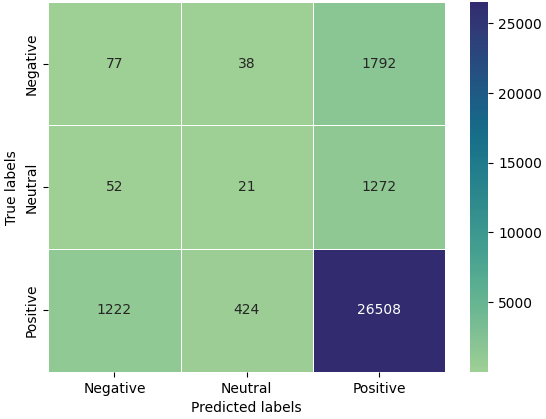
\includegraphics[scale=0.5]{images/conf_mat.PNG}
%     \caption{Confusion Matrix for Bangla-BERT}
%     \label{fig:conf_matrix}
% \end{figure}
% %%%%%%%%%%%%%%%%%%%%%%%%%%%%%%%%%%%%%%%%%%%%%%%%%%%






\section{Morphology and Negation Patterns of Bangla}
% EXAMPLES DEWA LAGBE
Understanding the morphology and negation patterns of a language holds paramount importance in the realm of sentiment analysis because negation can alter the meaning of words and phrases, thereby affecting the overall sentiment conveyed by a text. We provide a concise yet insightful recapitulation of the topic in the case of Bangla accompanied by review samples from our dataset \textsc{BanglaBook} as the respective examples. From the linguistic typological standpoint, Bangla is categorized as a \textit{subject-object-verb} (SOV) language because the subject, object, and verb generally adhere to said order in its sentential structure \cite{ramchand2004two}. The most common juxtaposition of polarity from positive to negative is the use of \textit{ni} ($\text{\bangla নি}$) as a tensed negative. For example,
\vspace{-5pt}
\begin{quote}
\centering
    $\text{\smallbangla আমি তাঁর অনুরাগী হওয়ায় আমি এই বইটি কেনা}$\\$\text{\smallbangla থেকে নিজেকে প্রতিরোধ করতে \colorbox{red!30}{পারিনি}!!!!}$\\
    \small \textbf{Translation:} As I am a fan of his I \colorbox{red!30}{couldn't} resist myself from buying this book!!!!
\end{quote}
% \vspace{-3pt}
Another negational feature is expressed by placing \textit{na} ($\text{\bangla না}$) prior to the non-finite verb and after the finite verb in a sentence (although there are some exceptions). For example,
\vspace{-7pt}
\begin{quote}
\centering
    $\text{\smallbangla অবশ্য হুমায়ুন আহমেদ লিখেছেন এই বইটার}$\\$\text{\smallbangla উপরে তিনি নিজেও সন্তুষ্ট \colorbox{red!30}{না}।}$\\
    \small \textbf{Translation:} Of course, Humayun Ahmed wrote that he himself is \colorbox{red!30}{not} satisfied with this book.
\end{quote}
The Bangla language consists of no negative adverbs or pronouns \cite{thompson2006negation}. This is why the negative element responsible for the reversal of polarity transcends from the word-level to the sentence-level rendering the occurrences of almost all negations in Bangla manifest on the syntactic level \cite{thompson2006negation}. 

In the cases of double negatives, we see the involvement of lexical negation, a morphological feature that works with negative affixes (prefixes and suffixes) attached to a root word. The prefixes in Bangla have two different phonetic variations or allophones depending on whether the prefix precedes a vowel or a consonant. The same is true for prefixes that imbue a negative connotation to a root word, e.g. \textit{o} ($\text{\bangla অ}$) and \textit{on} ($\text{\bangla অন্‌}$). For example,
\vspace{-7pt}
\begin{quote}
\centering
    $\text{\smallbangla কিন্তু এই বইটি এই \colorbox{red!30}{অপূর্ণতা} ঢেকে ফেলেছে।}$\\
    \small \textbf{Translation:} But this book has covered up this \colorbox{red!30}{incompleteness}.\\
    \vspace{5pt}
    $\text{\smallbangla ওমর খৈয়ামের ভাষায় কিছু বই \colorbox{red!30}{অনন্ত} যৌবনের বই,}$\\$\text{\smallbangla যাদের কোন ক্ষয় নেই।}$\\
    \small \textbf{Translation:} In the words of Omar Khayyam, some books are books of \colorbox{red!30}{never-ending} youth, which have no decay.
\end{quote}
Another negative prefix that precedes a root word to invert its polarity is \textit{nir} ($\text{\smallbangla নির্‌}$). For example,
\vspace{-5pt}
\begin{quote}
    \centering
    $\text{\smallbangla লেখকের \colorbox{red!30}{নিরলস} শ্রম লেখায় ফুটে উঠেছে।}$\\
    \small \textbf{Translation:} The \colorbox{red!30}{relentless} effort of the author is reflected in the writing.
\end{quote}
On the contrary, the suffix \textit{hin} ($\text{\bangla হীন}$) succeeds a root word to convert it to the corresponding negative form. For example,
\vspace{-12pt}
\begin{quoting}
\centering
    $\text{\smallbangla এরকম \colorbox{red!30}{ভিত্তিহীন} কাল্পনিক গল্প শিশুদের না পড়াই ভালো।}$\\
    \small \textbf{Translation:} It is better for children not to read such \colorbox{red!30}{baseless} fictional stories.
\end{quoting}
The expression of negative sentiment is, therefore, very nuanced in the Bangla language as every occurrence of negative is intertwined with features like the tense, hierarchy of syntax, verb status, case-specific issues, and sequential arrangement of words \cite{thompson2006negation}.
\section{Conclusion}
This paper introduces \textsc{BanglaBook}, the largest Bangla book review dataset with 158,065 samples, each labeled with 1 of 3 user sentiments. We provide extensive statistical analysis and strong baselines facilitating the utility of the dataset. Given its massive size and fine-grained sentiment distribution, \textsc{BanglaBook} has the potential to alleviate the resource scarcity in Bangla language research.
\section{Limitations}
Many of the reviews that were gathered for constructing \textsc{BanglaBook} are discarded because they lack a corresponding rating. A manual annotation process would have yielded a much larger dataset, which was not feasible due to resource constraints. Moreover, one of the challenges for validating the dataset is the lack of statistical models and word-embeddings pre-trained on the Bangla language. Some pre-trained Bangla-BERT models, yet to be trained on extensive corpora, have only recently been proposed. Improving transformer-based models for Bangla can enhance sub-word level contextual understanding which will consequently help in more accurate identification of the sentiments in \textsc{BanglaBook} \cite{islam2022emonoba}.
%\section{Acknowledgements}
% THANK ALLAH, PARENTS, AND SSL
% \section{Introduction}

% These instructions are for authors submitting papers to ACL 2023 using \LaTeX. They are not self-contained. All authors must follow the general instructions for *ACL proceedings,\footnote{\url{http://acl-org.github.io/ACLPUB/formatting.html}} as well as guidelines set forth in the ACL 2023 call for papers.\footnote{\url{https://2023.aclweb.org/calls/main_conference/}} This document contains additional instructions for the \LaTeX{} style files.
% The templates include the \LaTeX{} source of this document (\texttt{acl2023.tex}),
% the \LaTeX{} style file used to format it (\texttt{acl2023.sty}),
% an ACL bibliography style (\texttt{acl\_natbib.bst}),
% an example bibliography (\texttt{custom.bib}),
% and the bibliography for the ACL Anthology (\texttt{anthology.bib}).

% \section{Engines}

% To produce a PDF file, pdf\LaTeX{} is strongly recommended (over original \LaTeX{} plus dvips+ps2pdf or dvipdf). Xe\LaTeX{} also produces PDF files, and is especially suitable for text in non-Latin scripts.
% \begin{table}
% \centering
% \begin{tabular}{lc}
% \hline
% \textbf{Command} & \textbf{Output}\\
% \hline
% \verb|{\"a}| & {\"a} \\
% \verb|{\^e}| & {\^e} \\
% \verb|{\`i}| & {\`i} \\ 
% \verb|{\.I}| & {\.I} \\ 
% \verb|{\o}| & {\o} \\
% \verb|{\'u}| & {\'u}  \\ 
% \verb|{\aa}| & {\aa}  \\\hline
% \end{tabular}
% \begin{tabular}{lc}
% \hline
% \textbf{Command} & \textbf{Output}\\
% \hline
% \verb|{\c c}| & {\c c} \\ 
% \verb|{\u g}| & {\u g} \\ 
% \verb|{\l}| & {\l} \\ 
% \verb|{\~n}| & {\~n} \\ 
% \verb|{\H o}| & {\H o} \\ 
% \verb|{\v r}| & {\v r} \\ 
% \verb|{\ss}| & {\ss} \\
% \hline
% \end{tabular}
% \caption{Example commands for accented characters, to be used in, \emph{e.g.}, Bib\TeX{} entries.}
% \label{tab:accents}
% \end{table}
% \section{Preamble}
% \begin{table*}
% \centering
% \begin{tabular}{lll}
% \hline
% \textbf{Output} & \textbf{natbib command} & \textbf{Old ACL-style command}\\
% \hline
% \citep{ct1965} & \verb|\citep| & \verb|\cite| \\
% \citealp{ct1965} & \verb|\citealp| & no equivalent \\
% \citet{ct1965} & \verb|\citet| & \verb|\newcite| \\
% \citeyearpar{ct1965} & \verb|\citeyearpar| & \verb|\shortcite| \\
% \citeposs{ct1965} & \verb|\citeposs| & no equivalent \\
% \citep[FFT;][]{ct1965} &  \verb|\citep[FFT;][]| & no equivalent\\
% \hline
% \end{tabular}
% \caption{\label{citation-guide}
% Citation commands supported by the style file.
% The style is based on the natbib package and supports all natbib citation commands.
% It also supports commands defined in previous ACL style files for compatibility.
% }
% \end{table*}
% The first line of the file must be
% \begin{quote}
% \begin{verbatim}
% \documentclass[11pt]{article}
% \end{verbatim}
% \end{quote}
% To load the style file in the review version:
% \begin{quote}
% \begin{verbatim}
% \usepackage[review]{ACL2023}
% \end{verbatim}
% \end{quote}
% For the final version, omit the \verb|review| option:
% \begin{quote}
% \begin{verbatim}
% \usepackage{ACL2023}
% \end{verbatim}
% \end{quote}
% To use Times Roman, put the following in the preamble:
% \begin{quote}
% \begin{verbatim}
% \usepackage{times}
% \end{verbatim}
% \end{quote}
% (Alternatives like txfonts or newtx are also acceptable.)
% Please see the \LaTeX{} source of this document for comments on other packages that may be useful.
% Set the title and author using \verb|\title| and \verb|\author|. Within the author list, format multiple authors using \verb|\and| and \verb|\And| and \verb|\AND|; please see the \LaTeX{} source for examples.
% By default, the box containing the title and author names is set to the minimum of 5 cm. If you need more space, include the following in the preamble:
% \begin{quote}
% \begin{verbatim}
% \setlength\titlebox{<dim>}
% \end{verbatim}
% \end{quote}
% where \verb|<dim>| is replaced with a length. Do not set this length smaller than 5 cm.

% \section{Document Body}

% \subsection{Footnotes}

% Footnotes are inserted with the \verb|\footnote| command.\footnote{This is a footnote.}

% \subsection{Tables and figures}

% See Table~\ref{tab:accents} for an example of a table and its caption.
% \textbf{Do not override the default caption sizes.}

% \subsection{Hyperlinks}

% Users of older versions of \LaTeX{} may encounter the following error during compilation: 
% \begin{quote}
% \tt\verb|\pdfendlink| ended up in different nesting level than \verb|\pdfstartlink|.
% \end{quote}
% This happens when pdf\LaTeX{} is used and a citation splits across a page boundary. The best way to fix this is to upgrade \LaTeX{} to 2018-12-01 or later.

% \subsection{Citations}



% Table~\ref{citation-guide} shows the syntax supported by the style files.
% We encourage you to use the natbib styles.
% You can use the command \verb|\citet| (cite in text) to get ``author (year)'' citations, like this citation to a paper by \citet{Gusfield:97}.
% You can use the command \verb|\citep| (cite in parentheses) to get ``(author, year)'' citations \citep{Gusfield:97}.
% You can use the command \verb|\citealp| (alternative cite without parentheses) to get ``author, year'' citations, which is useful for using citations within parentheses (e.g. \citealp{Gusfield:97}).

% \subsection{References}

% \nocite{Ando2005,augenstein-etal-2016-stance,andrew2007scalable,rasooli-tetrault-2015,goodman-etal-2016-noise,harper-2014-learning}

% The \LaTeX{} and Bib\TeX{} style files provided roughly follow the American Psychological Association format.
% If your own bib file is named \texttt{custom.bib}, then placing the following before any appendices in your \LaTeX{} file will generate the references section for you:
% \begin{quote}
% \begin{verbatim}
% \bibliographystyle{acl_natbib}
% \bibliography{custom}
% \end{verbatim}
% \end{quote}
% You can obtain the complete ACL Anthology as a Bib\TeX{} file from \url{https://aclweb.org/anthology/anthology.bib.gz}.
% To include both the Anthology and your own .bib file, use the following instead of the above.
% \begin{quote}
% \begin{verbatim}
% \bibliographystyle{acl_natbib}
% \bibliography{anthology,custom}
% \end{verbatim}
% \end{quote}
% Please see Section~\ref{sec:bibtex} for information on preparing Bib\TeX{} files.

% \subsection{Appendices}

% Use \verb|\appendix| before any appendix section to switch the section numbering over to letters. See Appendix~\ref{sec:appendix} for an example.

% \section{Bib\TeX{} Files}
% \label{sec:bibtex}

% Unicode cannot be used in Bib\TeX{} entries, and some ways of typing special characters can disrupt Bib\TeX's alphabetization. The recommended way of typing special characters is shown in Table~\ref{tab:accents}.

% Please ensure that Bib\TeX{} records contain DOIs or URLs when possible, and for all the ACL materials that you reference.
% Use the \verb|doi| field for DOIs and the \verb|url| field for URLs.
% If a Bib\TeX{} entry has a URL or DOI field, the paper title in the references section will appear as a hyperlink to the paper, using the hyperref \LaTeX{} package.

% \section*{Limitations}
% ACL 2023 requires all submissions to have a section titled ``Limitations'', for discussing the limitations of the paper as a complement to the discussion of strengths in the main text. This section should occur after the conclusion, but before the references. It will not count towards the page limit.
% The discussion of limitations is mandatory. Papers without a limitation section will be desk-rejected without review.

% While we are open to different types of limitations, just mentioning that a set of results have been shown for English only probably does not reflect what we expect. 
% Mentioning that the method works mostly for languages with limited morphology, like English, is a much better alternative.
% In addition, limitations such as low scalability to long text, the requirement of large GPU resources, or other things that inspire crucial further investigation are welcome.

% \section*{Ethics Statement}
% Scientific work published at ACL 2023 must comply with the ACL Ethics Policy.\footnote{\url{https://www.aclweb.org/portal/content/acl-code-ethics}} We encourage all authors to include an explicit ethics statement on the broader impact of the work, or other ethical considerations after the conclusion but before the references. The ethics statement will not count toward the page limit (8 pages for long, 4 pages for short papers).

% \section*{Acknowledgements}
% This document has been adapted by Jordan Boyd-Graber, Naoaki Okazaki, Anna Rogers from the style files used for earlier ACL, EMNLP and NAACL proceedings, including those for
% EACL 2023 by Isabelle Augenstein and Andreas Vlachos,
% EMNLP 2022 by Yue Zhang, Ryan Cotterell and Lea Frermann,
% ACL 2020 by Steven Bethard, Ryan Cotterell and Rui Yan,
% ACL 2019 by Douwe Kiela and Ivan Vuli\'{c},
% NAACL 2019 by Stephanie Lukin and Alla Roskovskaya, 
% ACL 2018 by Shay Cohen, Kevin Gimpel, and Wei Lu, 
% NAACL 2018 by Margaret Mitchell and Stephanie Lukin,
% Bib\TeX{} suggestions for (NA)ACL 2017/2018 from Jason Eisner,
% ACL 2017 by Dan Gildea and Min-Yen Kan, NAACL 2017 by Margaret Mitchell, 
% ACL 2012 by Maggie Li and Michael White, 
% ACL 2010 by Jing-Shin Chang and Philipp Koehn, 
% ACL 2008 by Johanna D. Moore, Simone Teufel, James Allan, and Sadaoki Furui, 
% ACL 2005 by Hwee Tou Ng and Kemal Oflazer, 
% ACL 2002 by Eugene Charniak and Dekang Lin, 
% and earlier ACL and EACL formats written by several people, including
% John Chen, Henry S. Thompson and Donald Walker.
% Additional elements were taken from the formatting instructions of the \emph{International Joint Conference on Artificial Intelligence} and the \emph{Conference on Computer Vision and Pattern Recognition}.

% Entries for the entire Anthology, followed by custom entries
\newpage
\bibliography{anthology,custom}
\bibliographystyle{acl_natbib}

\appendix

\section{Appendix}
\label{sec:appendix}

% Please add the following required packages to your document preamble:
% \usepackage[table,xcdraw]{xcolor}
% If you use beamer only pass "xcolor=table" option, i.e. \documentclass[xcolor=table]{beamer}
% Tentative columns
% Dataset | sentiment | row for each sentiment | # of samples for each sentiment | Total | Availability | Sources | Benchmark models
% \begin{table*}[h]
% \centering
% \small
% \begin{tabular}{
% >{\columncolor[HTML]{FFFFFF}}c |
% >{\columncolor[HTML]{FFFFFF}}c }
% \hline
% \textbf{Dataset} & \textbf{\# of Samples} \\ \hline
% \cite{tabassum2019design} & 1,050 \\
% \cite{chowdhury2014performing} & 1,300 \\
% \cite{nabi2016detecting} & 1,500 \\
% \cite{mahtab2018sentiment} & 1,601 \\
% \cite{akter2016sentiment} & 3,600 \\
% \cite{dey2019sentiment} & 5,200 \\
% \cite{khatun2022machine} & 5,500 \\
% \cite{tuhin2019automated} & 7,500 \\
% \cite{akter2021bengali} & 7,905 \\
% \cite{hassan2016sentiment} & 9,337 \\
% \cite{rahib2022emotion} & 10,581 \\
% \cite{al2021social} & 11,006 \\
% \cite{sazzed2020development} & 12,000 \\
% \textsc{SentNoB}\cite{islam2021sentnob} & 15,728 \\
% \cite{islam2020sentiment} & 17,852 \\
% \textsc{EmoNoBa}\cite{islam2022emonoba} & 22,698 \\ \hline
% \textsc{BanglaBook} (ours) & \textbf{158,065} \\ \hline
% \end{tabular}
% \caption{Comparison of Bangla Sentiment Analysis datasets sorted in ascending order of size.}
% \label{tab:dataset_comparison}
% \end{table*}
%----------------------------------------------------------------
% Please add the following required packages to your document preamble:
% \usepackage{multirow}
% \usepackage[table,xcdraw]{xcolor}
% If you use beamer only pass "xcolor=table" option, i.e. \documentclass[xcolor=table]{beamer}
% \usepackage[normalem]{ulem}
% \useunder{\uline}{\ul}{}
\begin{table*}[h]
% \noindent
\centering
\tiny
% \makebox[\textwidth]{
\begin{tabular}{
>{\columncolor[HTML]{FFFFFF}}c |
>{\columncolor[HTML]{FFFFFF}}c 
>{\columncolor[HTML]{FFFFFF}}c |
>{\columncolor[HTML]{FFFFFF}}c 
>{\columncolor[HTML]{FFFFFF}}c |
>{\columncolor[HTML]{FFFFFF}}c |
>{\columncolor[HTML]{FFFFFF}}c |
>{\columncolor[HTML]{FFFFFF}}C{1cm} |
>{\columncolor[HTML]{FFFFFF}}c |
>{\columncolor[HTML]{FFFFFF}}c }
\hline
\cellcolor[HTML]{FFFFFF}{\color[HTML]{000000} } & \multicolumn{2}{c|}{\cellcolor[HTML]{FFFFFF}{\color[HTML]{000000} }} & \multicolumn{2}{c|}{\cellcolor[HTML]{FFFFFF}{\color[HTML]{000000} }} & \cellcolor[HTML]{FFFFFF}{\color[HTML]{000000} } & \cellcolor[HTML]{FFFFFF}{\color[HTML]{000000} } & \cellcolor[HTML]{FFFFFF}{\color[HTML]{000000} } & \cellcolor[HTML]{FFFFFF}{\color[HTML]{000000} } & \cellcolor[HTML]{FFFFFF}{\color[HTML]{000000} } \\
\multirow{-2}{*}{\cellcolor[HTML]{FFFFFF}{\color[HTML]{000000} \textbf{Dataset}}} & \multicolumn{2}{c|}{\multirow{-2}{*}{\cellcolor[HTML]{FFFFFF}{\color[HTML]{000000} \textbf{\begin{tabular}[c]{@{}c@{}}Sentiment \\ Classification\end{tabular}}}}} & \multicolumn{2}{c|}{\multirow{-2}{*}{\cellcolor[HTML]{FFFFFF}{\color[HTML]{000000} \textbf{\begin{tabular}[c]{@{}c@{}}Sentiment \\ Distribution\end{tabular}}}}} & \multirow{-2}{*}{\cellcolor[HTML]{FFFFFF}{\color[HTML]{000000} \textbf{\begin{tabular}[c]{@{}c@{}}Total \# of \\ Samples\end{tabular}}}} & \multirow{-2}{*}{\cellcolor[HTML]{FFFFFF}{\color[HTML]{000000} \textbf{Availability}}} & \multirow{-2}{*}{\cellcolor[HTML]{FFFFFF}{\color[HTML]{000000} \textbf{\begin{tabular}[c]{@{}C{1cm}@{}} Type of \\ Content\end{tabular}}}} & \multirow{-2}{*}{\cellcolor[HTML]{FFFFFF}{\color[HTML]{000000} \textbf{Source(s)}}} & \multirow{-2}{*}{\cellcolor[HTML]{FFFFFF}{\color[HTML]{000000} \textbf{Baseline Models}}} \\ \hline
\cellcolor[HTML]{FFFFFF}{\color[HTML]{000000} } & \multicolumn{2}{c|}{\cellcolor[HTML]{FFFFFF}{\color[HTML]{000000} Positive}} & \multicolumn{2}{c|}{\cellcolor[HTML]{FFFFFF}{\color[HTML]{000000} -}} & \cellcolor[HTML]{FFFFFF}{\color[HTML]{000000} } & \cellcolor[HTML]{FFFFFF}{\color[HTML]{000000} } & \cellcolor[HTML]{FFFFFF}{\color[HTML]{000000} } & \cellcolor[HTML]{FFFFFF}{\color[HTML]{000000} } & \cellcolor[HTML]{FFFFFF}{\color[HTML]{000000} } \\ \cline{2-5}
\multirow{-2}{*}{\cellcolor[HTML]{FFFFFF}{\color[HTML]{000000} \cite{tabassum2019design}}} & \multicolumn{2}{c|}{\cellcolor[HTML]{FFFFFF}{\color[HTML]{000000} Negative}} & \multicolumn{2}{c|}{\cellcolor[HTML]{FFFFFF}{\color[HTML]{000000} -}} & \multirow{-2}{*}{\cellcolor[HTML]{FFFFFF}{\color[HTML]{000000} 1,050}} & \multirow{-2}{*}{\cellcolor[HTML]{FFFFFF}{\color[HTML]{000000} Closed}} & \multirow{-2}{*}{\cellcolor[HTML]{FFFFFF}{\color[HTML]{000000} \begin{tabular}[c]{@{}c@{}}Posts, \\ comments\end{tabular}}} & \multirow{-2}{*}{\cellcolor[HTML]{FFFFFF}{\color[HTML]{000000} \begin{tabular}[c]{@{}c@{}}Facebook,\\ Twitter\end{tabular}}} & \multirow{-2}{*}{\cellcolor[HTML]{FFFFFF}{\color[HTML]{000000} RF}} \\ \hline
\cellcolor[HTML]{FFFFFF}{\color[HTML]{000000} } & \multicolumn{2}{c|}{\cellcolor[HTML]{FFFFFF}{\color[HTML]{000000} Positive}} & \multicolumn{2}{c|}{\cellcolor[HTML]{FFFFFF}{\color[HTML]{000000} -}} & \cellcolor[HTML]{FFFFFF}{\color[HTML]{000000} } & \cellcolor[HTML]{FFFFFF}{\color[HTML]{000000} } & \cellcolor[HTML]{FFFFFF}{\color[HTML]{000000} } & \cellcolor[HTML]{FFFFFF}{\color[HTML]{000000} } & \cellcolor[HTML]{FFFFFF}{\color[HTML]{000000} } \\ \cline{2-5}
\multirow{-2}{*}{\cellcolor[HTML]{FFFFFF}{\color[HTML]{000000} \cite{chowdhury2014performing}}} & \multicolumn{2}{c|}{\cellcolor[HTML]{FFFFFF}{\color[HTML]{000000} Negative}} & \multicolumn{2}{c|}{\cellcolor[HTML]{FFFFFF}{\color[HTML]{000000} -}} & \multirow{-2}{*}{\cellcolor[HTML]{FFFFFF}{\color[HTML]{000000} 1,300}} & \multirow{-2}{*}{\cellcolor[HTML]{FFFFFF}{\color[HTML]{000000} Closed}} & \multirow{-2}{*}{\cellcolor[HTML]{FFFFFF}{\color[HTML]{000000} \begin{tabular}[c]{@{}c@{}}Posts, \\ comments\end{tabular}}} & \multirow{-2}{*}{\cellcolor[HTML]{FFFFFF}{\color[HTML]{000000} Twitter}} & \multirow{-2}{*}{\cellcolor[HTML]{FFFFFF}{\color[HTML]{000000} -}} \\ \hline
\cellcolor[HTML]{FFFFFF}{\color[HTML]{000000} } & \multicolumn{2}{c|}{\cellcolor[HTML]{FFFFFF}{\color[HTML]{000000} Positive}} & \multicolumn{2}{c|}{\cellcolor[HTML]{FFFFFF}{\color[HTML]{000000} -}} & \cellcolor[HTML]{FFFFFF}{\color[HTML]{000000} } & \cellcolor[HTML]{FFFFFF}{\color[HTML]{000000} } & \cellcolor[HTML]{FFFFFF}{\color[HTML]{000000} } & \cellcolor[HTML]{FFFFFF}{\color[HTML]{000000} } & \cellcolor[HTML]{FFFFFF}{\color[HTML]{000000} } \\ \cline{2-5}
\multirow{-2}{*}{\cellcolor[HTML]{FFFFFF}{\color[HTML]{000000} \cite{nabi2016detecting}}} & \multicolumn{2}{c|}{\cellcolor[HTML]{FFFFFF}{\color[HTML]{000000} Negative}} & \multicolumn{2}{c|}{\cellcolor[HTML]{FFFFFF}{\color[HTML]{000000} -}} & \multirow{-2}{*}{\cellcolor[HTML]{FFFFFF}{\color[HTML]{000000} 1,500}} & \multirow{-2}{*}{\cellcolor[HTML]{FFFFFF}{\color[HTML]{000000} Closed}} & \multirow{-2}{*}{\cellcolor[HTML]{FFFFFF}{\color[HTML]{000000} \begin{tabular}[c]{@{}c@{}}Posts, \\ comments\end{tabular}}} & \multirow{-2}{*}{\cellcolor[HTML]{FFFFFF}{\color[HTML]{000000} Social Media}} & \multirow{-2}{*}{\cellcolor[HTML]{FFFFFF}{\color[HTML]{000000} -}} \\ \hline
\cellcolor[HTML]{FFFFFF}{\color[HTML]{000000} } & \multicolumn{2}{c|}{\cellcolor[HTML]{FFFFFF}{\color[HTML]{000000} Praise}} & \multicolumn{2}{c|}{\cellcolor[HTML]{FFFFFF}{\color[HTML]{000000} 513}} & \cellcolor[HTML]{FFFFFF}{\color[HTML]{000000} } & \cellcolor[HTML]{FFFFFF}{\color[HTML]{000000} } & \cellcolor[HTML]{FFFFFF}{\color[HTML]{000000} } & \cellcolor[HTML]{FFFFFF}{\color[HTML]{000000} } & \cellcolor[HTML]{FFFFFF}{\color[HTML]{000000} } \\ \cline{2-5}
\cellcolor[HTML]{FFFFFF}{\color[HTML]{000000} } & \multicolumn{2}{c|}{\cellcolor[HTML]{FFFFFF}{\color[HTML]{000000} Criticism}} & \multicolumn{2}{c|}{\cellcolor[HTML]{FFFFFF}{\color[HTML]{000000} 604}} & \cellcolor[HTML]{FFFFFF}{\color[HTML]{000000} } & \cellcolor[HTML]{FFFFFF}{\color[HTML]{000000} } & \cellcolor[HTML]{FFFFFF}{\color[HTML]{000000} } & \cellcolor[HTML]{FFFFFF}{\color[HTML]{000000} } & \cellcolor[HTML]{FFFFFF}{\color[HTML]{000000} } \\ \cline{2-5}
\multirow{-3}{*}{\cellcolor[HTML]{FFFFFF}{\color[HTML]{000000} \cite{mahtab2018sentiment}}} & \multicolumn{2}{c|}{\cellcolor[HTML]{FFFFFF}{\color[HTML]{000000} Sadness}} & \multicolumn{2}{c|}{\cellcolor[HTML]{FFFFFF}{\color[HTML]{000000} 484}} & \multirow{-3}{*}{\cellcolor[HTML]{FFFFFF}{\color[HTML]{000000} 1,601}} & \multirow{-3}{*}{\cellcolor[HTML]{FFFFFF}{\color[HTML]{000000} Closed}} & \multirow{-3}{*}{\cellcolor[HTML]{FFFFFF}{\color[HTML]{000000} Comments}} & \multirow{-3}{*}{\cellcolor[HTML]{FFFFFF}{\color[HTML]{000000} \begin{tabular}[c]{@{}c@{}}Prothom Alo \\ Online News \\ Portal\end{tabular}}} & \multirow{-3}{*}{\cellcolor[HTML]{FFFFFF}{\color[HTML]{000000} \begin{tabular}[c]{@{}c@{}}SVM, DT, \\ NB\end{tabular}}} \\ \hline
\cellcolor[HTML]{FFFFFF}{\color[HTML]{000000} } & \multicolumn{2}{c|}{\cellcolor[HTML]{FFFFFF}{\color[HTML]{000000} Positive}} & \multicolumn{2}{c|}{\cellcolor[HTML]{FFFFFF}{\color[HTML]{000000} -}} & \cellcolor[HTML]{FFFFFF}{\color[HTML]{000000} } & \cellcolor[HTML]{FFFFFF}{\color[HTML]{000000} } & \cellcolor[HTML]{FFFFFF}{\color[HTML]{000000} } & \cellcolor[HTML]{FFFFFF}{\color[HTML]{000000} } & \cellcolor[HTML]{FFFFFF}{\color[HTML]{000000} } \\ \cline{2-5}
\cellcolor[HTML]{FFFFFF}{\color[HTML]{000000} } & \multicolumn{2}{c|}{\cellcolor[HTML]{FFFFFF}{\color[HTML]{000000} Negative}} & \multicolumn{2}{c|}{\cellcolor[HTML]{FFFFFF}{\color[HTML]{000000} -}} & \cellcolor[HTML]{FFFFFF}{\color[HTML]{000000} } & \cellcolor[HTML]{FFFFFF}{\color[HTML]{000000} } & \cellcolor[HTML]{FFFFFF}{\color[HTML]{000000} } & \cellcolor[HTML]{FFFFFF}{\color[HTML]{000000} } & \cellcolor[HTML]{FFFFFF}{\color[HTML]{000000} } \\ \cline{2-5}
\multirow{-3}{*}{\cellcolor[HTML]{FFFFFF}{\color[HTML]{000000} \cite{akter2016sentiment}}} & \multicolumn{2}{c|}{\cellcolor[HTML]{FFFFFF}{\color[HTML]{000000} Neutral}} & \multicolumn{2}{c|}{\cellcolor[HTML]{FFFFFF}{\color[HTML]{000000} -}} & \multirow{-3}{*}{\cellcolor[HTML]{FFFFFF}{\color[HTML]{000000} 3,600}} & \multirow{-3}{*}{\cellcolor[HTML]{FFFFFF}{\color[HTML]{000000} Closed}} & \multirow{-3}{*}{\cellcolor[HTML]{FFFFFF}{\color[HTML]{000000} \begin{tabular}[c]{@{}c@{}}Posts, \\ comments\end{tabular}}} & \multirow{-3}{*}{\cellcolor[HTML]{FFFFFF}{\color[HTML]{000000} Facebook}} & \multirow{-3}{*}{\cellcolor[HTML]{FFFFFF}{\color[HTML]{000000} NB}} \\ \hline
\cellcolor[HTML]{FFFFFF}{\color[HTML]{000000} } & \multicolumn{2}{c|}{\cellcolor[HTML]{FFFFFF}{\color[HTML]{000000} Positive}} & \multicolumn{2}{c|}{\cellcolor[HTML]{FFFFFF}{\color[HTML]{000000} -}} & \cellcolor[HTML]{FFFFFF}{\color[HTML]{000000} } & \cellcolor[HTML]{FFFFFF}{\color[HTML]{000000} } & \cellcolor[HTML]{FFFFFF}{\color[HTML]{000000} } & \cellcolor[HTML]{FFFFFF}{\color[HTML]{000000} } & \cellcolor[HTML]{FFFFFF}{\color[HTML]{000000} } \\ \cline{2-5}
\cellcolor[HTML]{FFFFFF}{\color[HTML]{000000} } & \multicolumn{2}{c|}{\cellcolor[HTML]{FFFFFF}{\color[HTML]{000000} Negative}} & \multicolumn{2}{c|}{\cellcolor[HTML]{FFFFFF}{\color[HTML]{000000} -}} & \cellcolor[HTML]{FFFFFF}{\color[HTML]{000000} } & \cellcolor[HTML]{FFFFFF}{\color[HTML]{000000} } & \cellcolor[HTML]{FFFFFF}{\color[HTML]{000000} } & \cellcolor[HTML]{FFFFFF}{\color[HTML]{000000} } & \cellcolor[HTML]{FFFFFF}{\color[HTML]{000000} } \\ \cline{2-5}
\multirow{-3}{*}{\cellcolor[HTML]{FFFFFF}{\color[HTML]{000000} \cite{rahman2018datasets}}} & \multicolumn{2}{c|}{\cellcolor[HTML]{FFFFFF}{\color[HTML]{000000} Neutral}} & \multicolumn{2}{c|}{\cellcolor[HTML]{FFFFFF}{\color[HTML]{000000} -}} & \multirow{-3}{*}{\cellcolor[HTML]{FFFFFF}{\color[HTML]{000000} 4,700}} & \multirow{-3}{*}{\cellcolor[HTML]{FFFFFF}{\color[HTML]{000000} \href{https://github.com/atik-05/Bangla_ABSA_Datasets}{\textbf{Open}}}} & \multirow{-3}{*}{\cellcolor[HTML]{FFFFFF}{\color[HTML]{000000} Comments}} & \multirow{-3}{*}{\cellcolor[HTML]{FFFFFF}{\color[HTML]{000000} \begin{tabular}[c]{@{}c@{}}Facebook pages: \\ BBC Bangla, \\ Prothom Alo\end{tabular}}} & \multirow{-3}{*}{\cellcolor[HTML]{FFFFFF}{\color[HTML]{000000} \begin{tabular}[c]{@{}c@{}}SVM, LR, KNN, \\ DT, LSTM \\ NB, CNN\end{tabular}}} \\ \hline
\cellcolor[HTML]{FFFFFF}{\color[HTML]{000000} } & \multicolumn{2}{c|}{\cellcolor[HTML]{FFFFFF}{\color[HTML]{000000} Positive}} & \multicolumn{2}{c|}{\cellcolor[HTML]{FFFFFF}{\color[HTML]{000000} 2,600}} & \cellcolor[HTML]{FFFFFF}{\color[HTML]{000000} } & \cellcolor[HTML]{FFFFFF}{\color[HTML]{000000} } & \cellcolor[HTML]{FFFFFF}{\color[HTML]{000000} } & \cellcolor[HTML]{FFFFFF}{\color[HTML]{000000} } & \cellcolor[HTML]{FFFFFF}{\color[HTML]{000000} } \\ \cline{2-5}
\multirow{-2}{*}{\cellcolor[HTML]{FFFFFF}{\color[HTML]{000000} \cite{dey2019sentiment}}} & \multicolumn{2}{c|}{\cellcolor[HTML]{FFFFFF}{\color[HTML]{000000} Negative}} & \multicolumn{2}{c|}{\cellcolor[HTML]{FFFFFF}{\color[HTML]{000000} 2,600}} & \multirow{-2}{*}{\cellcolor[HTML]{FFFFFF}{\color[HTML]{000000} 5,200}} & \multirow{-2}{*}{\cellcolor[HTML]{FFFFFF}{\color[HTML]{000000} Closed}} & \multirow{-2}{*}{\cellcolor[HTML]{FFFFFF}{\color[HTML]{000000} \begin{tabular}[c]{@{}c@{}}Comments,\\ reviews\end{tabular}}} & \multirow{-2}{*}{\cellcolor[HTML]{FFFFFF}{\color[HTML]{000000} \begin{tabular}[c]{@{}c@{}}Facebook, Twitter, \\ YouTube, News Portals\end{tabular}}} & \multirow{-2}{*}{\cellcolor[HTML]{FFFFFF}{\color[HTML]{000000} \begin{tabular}[c]{@{}c@{}}DT, \\ NB, SVM\end{tabular}}} \\ \hline
\cellcolor[HTML]{FFFFFF}{\color[HTML]{000000} } & \multicolumn{2}{c|}{\cellcolor[HTML]{FFFFFF}{\color[HTML]{000000} Positive}} & \multicolumn{2}{c|}{\cellcolor[HTML]{FFFFFF}{\color[HTML]{000000} -}} & \cellcolor[HTML]{FFFFFF}{\color[HTML]{000000} } & \cellcolor[HTML]{FFFFFF}{\color[HTML]{000000} } & \cellcolor[HTML]{FFFFFF}{\color[HTML]{000000} } & \cellcolor[HTML]{FFFFFF}{\color[HTML]{000000} } & \cellcolor[HTML]{FFFFFF}{\color[HTML]{000000} } \\ \cline{2-5}
\multirow{-2}{*}{\cellcolor[HTML]{FFFFFF}{\color[HTML]{000000} \cite{khatun2022machine}}} & \multicolumn{2}{c|}{\cellcolor[HTML]{FFFFFF}{\color[HTML]{000000} Negative}} & \multicolumn{2}{c|}{\cellcolor[HTML]{FFFFFF}{\color[HTML]{000000} -}} & \multirow{-2}{*}{\cellcolor[HTML]{FFFFFF}{\color[HTML]{000000} 5,500}} & \multirow{-2}{*}{\cellcolor[HTML]{FFFFFF}{\color[HTML]{000000} Closed}} & \multirow{-2}{*}{\cellcolor[HTML]{FFFFFF}{\color[HTML]{000000} \begin{tabular}[c]{@{}c@{}}Comments, \\ reviews\end{tabular}}} & \multirow{-2}{*}{\cellcolor[HTML]{FFFFFF}{\color[HTML]{000000} \begin{tabular}[c]{@{}c@{}}Social Media\end{tabular}}} & \multirow{-2}{*}{\cellcolor[HTML]{FFFFFF}{\color[HTML]{000000} \begin{tabular}[c]{@{}c@{}}-\end{tabular}}} \\ \hline
\cellcolor[HTML]{FFFFFF}{\color[HTML]{000000} } & \multicolumn{2}{c|}{\cellcolor[HTML]{FFFFFF}{\color[HTML]{000000} Anger}} & \multicolumn{2}{c|}{\cellcolor[HTML]{FFFFFF}{\color[HTML]{000000} -}} & \cellcolor[HTML]{FFFFFF}{\color[HTML]{000000} } & \cellcolor[HTML]{FFFFFF}{\color[HTML]{000000} } & \cellcolor[HTML]{FFFFFF}{\color[HTML]{000000} } & \cellcolor[HTML]{FFFFFF}{\color[HTML]{000000} } & \cellcolor[HTML]{FFFFFF}{\color[HTML]{000000} } \\ \cline{2-5}
\cellcolor[HTML]{FFFFFF}{\color[HTML]{000000} } & \multicolumn{2}{c|}{\cellcolor[HTML]{FFFFFF}{\color[HTML]{000000} Fear}} & \multicolumn{2}{c|}{\cellcolor[HTML]{FFFFFF}{\color[HTML]{000000} -}} & \cellcolor[HTML]{FFFFFF}{\color[HTML]{000000} } & \cellcolor[HTML]{FFFFFF}{\color[HTML]{000000} } & \cellcolor[HTML]{FFFFFF}{\color[HTML]{000000} } & \cellcolor[HTML]{FFFFFF}{\color[HTML]{000000} } & \cellcolor[HTML]{FFFFFF}{\color[HTML]{000000} } \\ \cline{2-5}
\cellcolor[HTML]{FFFFFF}{\color[HTML]{000000} } & \multicolumn{2}{c|}{\cellcolor[HTML]{FFFFFF}{\color[HTML]{000000} Surprise}} & \multicolumn{2}{c|}{\cellcolor[HTML]{FFFFFF}{\color[HTML]{000000} -}} & \cellcolor[HTML]{FFFFFF}{\color[HTML]{000000} } & \cellcolor[HTML]{FFFFFF}{\color[HTML]{000000} } & \cellcolor[HTML]{FFFFFF}{\color[HTML]{000000} } & \cellcolor[HTML]{FFFFFF}{\color[HTML]{000000} } & \cellcolor[HTML]{FFFFFF}{\color[HTML]{000000} } \\ \cline{2-5}
\cellcolor[HTML]{FFFFFF}{\color[HTML]{000000} } & \multicolumn{2}{c|}{\cellcolor[HTML]{FFFFFF}{\color[HTML]{000000} Sadness}} & \multicolumn{2}{c|}{\cellcolor[HTML]{FFFFFF}{\color[HTML]{000000} -}} & \cellcolor[HTML]{FFFFFF}{\color[HTML]{000000} } & \cellcolor[HTML]{FFFFFF}{\color[HTML]{000000} } & \cellcolor[HTML]{FFFFFF}{\color[HTML]{000000} } & \cellcolor[HTML]{FFFFFF}{\color[HTML]{000000} } & \cellcolor[HTML]{FFFFFF}{\color[HTML]{000000} } \\ \cline{2-5}
\cellcolor[HTML]{FFFFFF}{\color[HTML]{000000} } & \multicolumn{2}{c|}{\cellcolor[HTML]{FFFFFF}{\color[HTML]{000000} Joy}} & \multicolumn{2}{c|}{\cellcolor[HTML]{FFFFFF}{\color[HTML]{000000} -}} & \cellcolor[HTML]{FFFFFF}{\color[HTML]{000000} } & \cellcolor[HTML]{FFFFFF}{\color[HTML]{000000} } & \cellcolor[HTML]{FFFFFF}{\color[HTML]{000000} } & \cellcolor[HTML]{FFFFFF}{\color[HTML]{000000} } & \cellcolor[HTML]{FFFFFF}{\color[HTML]{000000} } \\ \cline{2-5}
\multirow{-6}{*}{\cellcolor[HTML]{FFFFFF}{\color[HTML]{000000} \textsc{BEmoC} \cite{iqbal2022bemoc}}} & \multicolumn{2}{c|}{\cellcolor[HTML]{FFFFFF}{\color[HTML]{000000} Disgust}} & \multicolumn{2}{c|}{\cellcolor[HTML]{FFFFFF}{\color[HTML]{000000} -}} & \multirow{-6}{*}{\cellcolor[HTML]{FFFFFF}{\color[HTML]{000000} 7,000}} & \multirow{-6}{*}{\cellcolor[HTML]{FFFFFF}{\color[HTML]{000000} \href{https://github.com/avishek-018/BEmoC-Bengali-Emotion-Courpus}{\textbf{Open}}}} & \multirow{-6}{*}{\cellcolor[HTML]{FFFFFF}{\color[HTML]{000000} \begin{tabular}[c]{@{}c@{}}Posts, \\ comments\end{tabular}}} & \multirow{-6}{*}{\cellcolor[HTML]{FFFFFF}{\color[HTML]{000000} \begin{tabular}[c]{@{}c@{}}Facebook, YouTube, \\ Online blogs, \\ Bangla story \\ books, novels, \\ newspapers,\\ discourse\end{tabular}}} & \multirow{-6}{*}{\cellcolor[HTML]{FFFFFF}{\color[HTML]{000000} -}} \\ \hline
\cellcolor[HTML]{FFFFFF}{\color[HTML]{000000} } & \multicolumn{2}{c|}{\cellcolor[HTML]{FFFFFF}{\color[HTML]{000000} Happy}} & \multicolumn{2}{c|}{\cellcolor[HTML]{FFFFFF}{\color[HTML]{000000} -}} & \cellcolor[HTML]{FFFFFF}{\color[HTML]{000000} } & \cellcolor[HTML]{FFFFFF}{\color[HTML]{000000} } & \cellcolor[HTML]{FFFFFF}{\color[HTML]{000000} } & \cellcolor[HTML]{FFFFFF}{\color[HTML]{000000} } & \cellcolor[HTML]{FFFFFF}{\color[HTML]{000000} } \\ \cline{2-5}
\cellcolor[HTML]{FFFFFF}{\color[HTML]{000000} } & \multicolumn{2}{c|}{\cellcolor[HTML]{FFFFFF}{\color[HTML]{000000} Tender}} & \multicolumn{2}{c|}{\cellcolor[HTML]{FFFFFF}{\color[HTML]{000000} -}} & \cellcolor[HTML]{FFFFFF}{\color[HTML]{000000} } & \cellcolor[HTML]{FFFFFF}{\color[HTML]{000000} } & \cellcolor[HTML]{FFFFFF}{\color[HTML]{000000} } & \cellcolor[HTML]{FFFFFF}{\color[HTML]{000000} } & \cellcolor[HTML]{FFFFFF}{\color[HTML]{000000} } \\ \cline{2-5}
\cellcolor[HTML]{FFFFFF}{\color[HTML]{000000} } & \multicolumn{2}{c|}{\cellcolor[HTML]{FFFFFF}{\color[HTML]{000000} Excited}} & \multicolumn{2}{c|}{\cellcolor[HTML]{FFFFFF}{\color[HTML]{000000} -}} & \cellcolor[HTML]{FFFFFF}{\color[HTML]{000000} } & \cellcolor[HTML]{FFFFFF}{\color[HTML]{000000} } & \cellcolor[HTML]{FFFFFF}{\color[HTML]{000000} } & \cellcolor[HTML]{FFFFFF}{\color[HTML]{000000} } & \cellcolor[HTML]{FFFFFF}{\color[HTML]{000000} } \\ \cline{2-5}
\cellcolor[HTML]{FFFFFF}{\color[HTML]{000000} } & \multicolumn{2}{c|}{\cellcolor[HTML]{FFFFFF}{\color[HTML]{000000} Sad}} & \multicolumn{2}{c|}{\cellcolor[HTML]{FFFFFF}{\color[HTML]{000000} -}} & \cellcolor[HTML]{FFFFFF}{\color[HTML]{000000} } & \cellcolor[HTML]{FFFFFF}{\color[HTML]{000000} } & \cellcolor[HTML]{FFFFFF}{\color[HTML]{000000} } & \cellcolor[HTML]{FFFFFF}{\color[HTML]{000000} } & \cellcolor[HTML]{FFFFFF}{\color[HTML]{000000} } \\ \cline{2-5}
\cellcolor[HTML]{FFFFFF}{\color[HTML]{000000} } & \multicolumn{2}{c|}{\cellcolor[HTML]{FFFFFF}{\color[HTML]{000000} Angry}} & \multicolumn{2}{c|}{\cellcolor[HTML]{FFFFFF}{\color[HTML]{000000} -}} & \cellcolor[HTML]{FFFFFF}{\color[HTML]{000000} } & \cellcolor[HTML]{FFFFFF}{\color[HTML]{000000} } & \cellcolor[HTML]{FFFFFF}{\color[HTML]{000000} } & \cellcolor[HTML]{FFFFFF}{\color[HTML]{000000} } & \cellcolor[HTML]{FFFFFF}{\color[HTML]{000000} } \\ \cline{2-5}
\multirow{-6}{*}{\cellcolor[HTML]{FFFFFF}{\color[HTML]{000000} \cite{tuhin2019automated}}} & \multicolumn{2}{c|}{\cellcolor[HTML]{FFFFFF}{\color[HTML]{000000} Scared}} & \multicolumn{2}{c|}{\cellcolor[HTML]{FFFFFF}{\color[HTML]{000000} -}} & \multirow{-6}{*}{\cellcolor[HTML]{FFFFFF}{\color[HTML]{000000} 7,500}} & \multirow{-6}{*}{\cellcolor[HTML]{FFFFFF}{\color[HTML]{000000} Closed}} & \multirow{-6}{*}{\cellcolor[HTML]{FFFFFF}{\color[HTML]{000000} -}} & \multirow{-6}{*}{\cellcolor[HTML]{FFFFFF}{\color[HTML]{000000} -}} & \multirow{-6}{*}{\cellcolor[HTML]{FFFFFF}{\color[HTML]{000000} \begin{tabular}[c]{@{}c@{}}NB, \\ Tropical Method\end{tabular}}} \\ \hline
\cellcolor[HTML]{FFFFFF}{\color[HTML]{000000} } & \multicolumn{2}{c|}{\cellcolor[HTML]{FFFFFF}{\color[HTML]{000000} Positive}} & \multicolumn{2}{c|}{\cellcolor[HTML]{FFFFFF}{\color[HTML]{000000} -}} & \cellcolor[HTML]{FFFFFF}{\color[HTML]{000000} } & \cellcolor[HTML]{FFFFFF}{\color[HTML]{000000} } & \cellcolor[HTML]{FFFFFF}{\color[HTML]{000000} } & \cellcolor[HTML]{FFFFFF}{\color[HTML]{000000} } & \cellcolor[HTML]{FFFFFF}{\color[HTML]{000000} } \\ \cline{2-5}
\cellcolor[HTML]{FFFFFF}{\color[HTML]{000000} } & \multicolumn{2}{c|}{\cellcolor[HTML]{FFFFFF}{\color[HTML]{000000} Negative}} & \multicolumn{2}{c|}{\cellcolor[HTML]{FFFFFF}{\color[HTML]{000000} -}} & \cellcolor[HTML]{FFFFFF}{\color[HTML]{000000} } & \cellcolor[HTML]{FFFFFF}{\color[HTML]{000000} } & \cellcolor[HTML]{FFFFFF}{\color[HTML]{000000} } & \cellcolor[HTML]{FFFFFF}{\color[HTML]{000000} } & \cellcolor[HTML]{FFFFFF}{\color[HTML]{000000} } \\ \cline{2-5}
\multirow{-3}{*}{\cellcolor[HTML]{FFFFFF}{\color[HTML]{000000} \cite{akter2021bengali}}} & \multicolumn{2}{c|}{\cellcolor[HTML]{FFFFFF}{\color[HTML]{000000} Neutral}} & \multicolumn{2}{c|}{\cellcolor[HTML]{FFFFFF}{\color[HTML]{000000} -}} & \multirow{-3}{*}{\cellcolor[HTML]{FFFFFF}{\color[HTML]{000000} 7,905}} & \multirow{-3}{*}{\cellcolor[HTML]{FFFFFF}{\color[HTML]{000000} Closed}} & \multirow{-3}{*}{\cellcolor[HTML]{FFFFFF}{\color[HTML]{000000} \begin{tabular}[c]{@{}c@{}}Product \\ reviews\end{tabular}}} & \multirow{-3}{*}{\cellcolor[HTML]{FFFFFF}{\color[HTML]{000000} Daraz}} & \multirow{-3}{*}{\cellcolor[HTML]{FFFFFF}{\color[HTML]{000000} \begin{tabular}[c]{@{}c@{}}RF, LR, \\ SVM, KNN, \\XGB\end{tabular}}} \\ \hline
\cellcolor[HTML]{FFFFFF}{\color[HTML]{000000} } & \multicolumn{2}{c|}{\cellcolor[HTML]{FFFFFF}{\color[HTML]{000000} Positive}} & \multicolumn{2}{c|}{\cellcolor[HTML]{FFFFFF}{\color[HTML]{000000} -}} & \cellcolor[HTML]{FFFFFF}{\color[HTML]{000000} } & \cellcolor[HTML]{FFFFFF}{\color[HTML]{000000} } & \cellcolor[HTML]{FFFFFF}{\color[HTML]{000000} } & \cellcolor[HTML]{FFFFFF}{\color[HTML]{000000} } & \cellcolor[HTML]{FFFFFF}{\color[HTML]{000000} } \\ \cline{2-5}
\cellcolor[HTML]{FFFFFF}{\color[HTML]{000000} } & \multicolumn{2}{c|}{\cellcolor[HTML]{FFFFFF}{\color[HTML]{000000} Negative}} & \multicolumn{2}{c|}{\cellcolor[HTML]{FFFFFF}{\color[HTML]{000000} -}} & \cellcolor[HTML]{FFFFFF}{\color[HTML]{000000} } & \cellcolor[HTML]{FFFFFF}{\color[HTML]{000000} } & \cellcolor[HTML]{FFFFFF}{\color[HTML]{000000} } & \cellcolor[HTML]{FFFFFF}{\color[HTML]{000000} } & \cellcolor[HTML]{FFFFFF}{\color[HTML]{000000} } \\ \cline{2-5}
\multirow{-3}{*}{\cellcolor[HTML]{FFFFFF}{\color[HTML]{000000} \cite{hassan2016sentiment}}} & \multicolumn{2}{c|}{\cellcolor[HTML]{FFFFFF}{\color[HTML]{000000} Ambiguous}} & \multicolumn{2}{c|}{\cellcolor[HTML]{FFFFFF}{\color[HTML]{000000} -}} & \multirow{-3}{*}{\cellcolor[HTML]{FFFFFF}{\color[HTML]{000000} 9,337}} & \multirow{-3}{*}{\cellcolor[HTML]{FFFFFF}{\color[HTML]{000000} Closed}} & \multirow{-3}{*}{\cellcolor[HTML]{FFFFFF}{\color[HTML]{000000} \begin{tabular}[c]{@{}c@{}}Comments,\\  reviews\end{tabular}}} & \multirow{-3}{*}{\cellcolor[HTML]{FFFFFF}{\color[HTML]{000000} \begin{tabular}[c]{@{}c@{}}Facebook, Twitter, \\ YouTube, News Portals\end{tabular}}} & \multirow{-3}{*}{\cellcolor[HTML]{FFFFFF}{\color[HTML]{000000} LSTM}} \\ \hline
\cellcolor[HTML]{FFFFFF}{\color[HTML]{000000} } & \multicolumn{2}{c|}{\cellcolor[HTML]{FFFFFF}{\color[HTML]{000000} Insightful}} & \multicolumn{2}{c|}{\cellcolor[HTML]{FFFFFF}{\color[HTML]{000000} 3,800}} & \cellcolor[HTML]{FFFFFF}{\color[HTML]{000000} } & \cellcolor[HTML]{FFFFFF}{\color[HTML]{000000} } & \cellcolor[HTML]{FFFFFF}{\color[HTML]{000000} } & \cellcolor[HTML]{FFFFFF}{\color[HTML]{000000} } & \cellcolor[HTML]{FFFFFF}{\color[HTML]{000000} } \\ \cline{2-5}
\cellcolor[HTML]{FFFFFF}{\color[HTML]{000000} } & \multicolumn{2}{c|}{\cellcolor[HTML]{FFFFFF}{\color[HTML]{000000} Curious}} & \multicolumn{2}{c|}{\cellcolor[HTML]{FFFFFF}{\color[HTML]{000000} 3,549}} & \cellcolor[HTML]{FFFFFF}{\color[HTML]{000000} } & \cellcolor[HTML]{FFFFFF}{\color[HTML]{000000} } & \cellcolor[HTML]{FFFFFF}{\color[HTML]{000000} } & \cellcolor[HTML]{FFFFFF}{\color[HTML]{000000} } & \cellcolor[HTML]{FFFFFF}{\color[HTML]{000000} } \\ \cline{2-5}
\multirow{-3}{*}{\cellcolor[HTML]{FFFFFF}{\color[HTML]{000000} \cite{rahib2022emotion}}} & \multicolumn{2}{c|}{\cellcolor[HTML]{FFFFFF}{\color[HTML]{000000} Gratitude}} & \multicolumn{2}{c|}{\cellcolor[HTML]{FFFFFF}{\color[HTML]{000000} 3,232}} & \multirow{-3}{*}{\cellcolor[HTML]{FFFFFF}{\color[HTML]{000000} 10,581}} & \multirow{-3}{*}{\cellcolor[HTML]{FFFFFF}{\color[HTML]{000000} Closed}} & \multirow{-3}{*}{\cellcolor[HTML]{FFFFFF}{\color[HTML]{000000} Comments}} & \multirow{-3}{*}{\cellcolor[HTML]{FFFFFF}{\color[HTML]{000000} Social Media}} & \multirow{-3}{*}{\cellcolor[HTML]{FFFFFF}{\color[HTML]{000000} \begin{tabular}[c]{@{}c@{}}SVM, RF, \\ CNN, LSTM\end{tabular}}} \\ \hline
\cellcolor[HTML]{FFFFFF}{\color[HTML]{000000} } & \multicolumn{1}{c|}{\cellcolor[HTML]{FFFFFF}{\color[HTML]{000000} }} & {\color[HTML]{000000} \begin{tabular}[c]{@{}c@{}}Wishful \\ Thinking\end{tabular}} & \multicolumn{1}{c|}{\cellcolor[HTML]{FFFFFF}{\color[HTML]{000000} 967}} & \cellcolor[HTML]{FFFFFF}{\color[HTML]{000000} } & \cellcolor[HTML]{FFFFFF}{\color[HTML]{000000} } & \cellcolor[HTML]{FFFFFF}{\color[HTML]{000000} } & \cellcolor[HTML]{FFFFFF}{\color[HTML]{000000} } & \cellcolor[HTML]{FFFFFF}{\color[HTML]{000000} } & \cellcolor[HTML]{FFFFFF}{\color[HTML]{000000} } \\ \cline{3-4}
\cellcolor[HTML]{FFFFFF}{\color[HTML]{000000} } & \multicolumn{1}{c|}{\multirow{-2}{*}{\cellcolor[HTML]{FFFFFF}{\color[HTML]{000000} Positive}}} & {\color[HTML]{000000} Appreciation} & \multicolumn{1}{c|}{\cellcolor[HTML]{FFFFFF}{\color[HTML]{000000} 942}} & \multirow{-2}{*}{\cellcolor[HTML]{FFFFFF}{\color[HTML]{000000} 1,909}} & \cellcolor[HTML]{FFFFFF}{\color[HTML]{000000} } & \cellcolor[HTML]{FFFFFF}{\color[HTML]{000000} } & \cellcolor[HTML]{FFFFFF}{\color[HTML]{000000} } & \cellcolor[HTML]{FFFFFF}{\color[HTML]{000000} } & \cellcolor[HTML]{FFFFFF}{\color[HTML]{000000} } \\ \cline{2-5}
\cellcolor[HTML]{FFFFFF}{\color[HTML]{000000} } & \multicolumn{1}{c|}{\cellcolor[HTML]{FFFFFF}{\color[HTML]{000000} }} & {\color[HTML]{000000} \begin{tabular}[c]{@{}c@{}}Gender-based \\ hate\end{tabular}} & \multicolumn{1}{c|}{\cellcolor[HTML]{FFFFFF}{\color[HTML]{000000} 525}} & \cellcolor[HTML]{FFFFFF}{\color[HTML]{000000} } & \cellcolor[HTML]{FFFFFF}{\color[HTML]{000000} } & \cellcolor[HTML]{FFFFFF}{\color[HTML]{000000} } & \cellcolor[HTML]{FFFFFF}{\color[HTML]{000000} } & \cellcolor[HTML]{FFFFFF}{\color[HTML]{000000} } & \cellcolor[HTML]{FFFFFF}{\color[HTML]{000000} } \\ \cline{3-4}
\cellcolor[HTML]{FFFFFF}{\color[HTML]{000000} } & \multicolumn{1}{c|}{\cellcolor[HTML]{FFFFFF}{\color[HTML]{000000} }} & {\color[HTML]{000000} Religious hate} & \multicolumn{1}{c|}{\cellcolor[HTML]{FFFFFF}{\color[HTML]{000000} 731}} & \cellcolor[HTML]{FFFFFF}{\color[HTML]{000000} } & \cellcolor[HTML]{FFFFFF}{\color[HTML]{000000} } & \cellcolor[HTML]{FFFFFF}{\color[HTML]{000000} } & \cellcolor[HTML]{FFFFFF}{\color[HTML]{000000} } & \cellcolor[HTML]{FFFFFF}{\color[HTML]{000000} } & \cellcolor[HTML]{FFFFFF}{\color[HTML]{000000} } \\ \cline{3-4}
\cellcolor[HTML]{FFFFFF}{\color[HTML]{000000} } & \multicolumn{1}{c|}{\cellcolor[HTML]{FFFFFF}{\color[HTML]{000000} }} & {\color[HTML]{000000} Political hate} & \multicolumn{1}{c|}{\cellcolor[HTML]{FFFFFF}{\color[HTML]{000000} 572}} & \cellcolor[HTML]{FFFFFF}{\color[HTML]{000000} } & \cellcolor[HTML]{FFFFFF}{\color[HTML]{000000} } & \cellcolor[HTML]{FFFFFF}{\color[HTML]{000000} } & \cellcolor[HTML]{FFFFFF}{\color[HTML]{000000} } & \cellcolor[HTML]{FFFFFF}{\color[HTML]{000000} } & \cellcolor[HTML]{FFFFFF}{\color[HTML]{000000} } \\ \cline{3-4}
\cellcolor[HTML]{FFFFFF}{\color[HTML]{000000} } & \multicolumn{1}{c|}{\cellcolor[HTML]{FFFFFF}{\color[HTML]{000000} }} & {\color[HTML]{000000} Personal hate} & \multicolumn{1}{c|}{\cellcolor[HTML]{FFFFFF}{\color[HTML]{000000} 1,995}} & \cellcolor[HTML]{FFFFFF}{\color[HTML]{000000} } & \cellcolor[HTML]{FFFFFF}{\color[HTML]{000000} } & \cellcolor[HTML]{FFFFFF}{\color[HTML]{000000} } & \cellcolor[HTML]{FFFFFF}{\color[HTML]{000000} } & \cellcolor[HTML]{FFFFFF}{\color[HTML]{000000} } & \cellcolor[HTML]{FFFFFF}{\color[HTML]{000000} } \\ \cline{3-4}
\cellcolor[HTML]{FFFFFF}{\color[HTML]{000000} } & \multicolumn{1}{c|}{\multirow{-5}{*}{\cellcolor[HTML]{FFFFFF}{\color[HTML]{000000} Negative}}} & {\color[HTML]{000000} Sarcasm} & \multicolumn{1}{c|}{\cellcolor[HTML]{FFFFFF}{\color[HTML]{000000} 1,414}} & \multirow{-5}{*}{\cellcolor[HTML]{FFFFFF}{\color[HTML]{000000} 5,237}} & \cellcolor[HTML]{FFFFFF}{\color[HTML]{000000} } & \cellcolor[HTML]{FFFFFF}{\color[HTML]{000000} } & \cellcolor[HTML]{FFFFFF}{\color[HTML]{000000} } & \cellcolor[HTML]{FFFFFF}{\color[HTML]{000000} } & \cellcolor[HTML]{FFFFFF}{\color[HTML]{000000} } \\ \cline{2-5}
\multirow{-8}{*}{\cellcolor[HTML]{FFFFFF}{\color[HTML]{000000} \cite{al2021social}}} & \multicolumn{1}{c|}{\cellcolor[HTML]{FFFFFF}{\color[HTML]{000000} Neutral}} & {\color[HTML]{000000} -} & \multicolumn{1}{c|}{\cellcolor[HTML]{FFFFFF}{\color[HTML]{000000} 3,860}} & {\color[HTML]{000000} 3,860} & \multirow{-8}{*}{\cellcolor[HTML]{FFFFFF}{\color[HTML]{000000} 11,006}} & \multirow{-8}{*}{\cellcolor[HTML]{FFFFFF}{\color[HTML]{000000} Closed}} & \multirow{-8}{*}{\cellcolor[HTML]{FFFFFF}{\color[HTML]{000000} Comments}} & \multirow{-8}{*}{\cellcolor[HTML]{FFFFFF}{\color[HTML]{000000} Facebook}} & \multirow{-8}{*}{\cellcolor[HTML]{FFFFFF}{\color[HTML]{000000} \begin{tabular}[c]{@{}c@{}}LR, DT, \\ RF, MNB, \\ KNN, \\ Linear SVM, \\ RBF SVM, \\ XGB\end{tabular}}} \\ \hline
\cellcolor[HTML]{FFFFFF}{\color[HTML]{000000} } & \multicolumn{2}{c|}{\cellcolor[HTML]{FFFFFF}{\color[HTML]{000000} Positive}} & \multicolumn{2}{c|}{\cellcolor[HTML]{FFFFFF}{\color[HTML]{000000} 8,500}} & \cellcolor[HTML]{FFFFFF}{\color[HTML]{000000} } & \cellcolor[HTML]{FFFFFF}{\color[HTML]{000000} } & \cellcolor[HTML]{FFFFFF}{\color[HTML]{000000} } & \cellcolor[HTML]{FFFFFF}{\color[HTML]{000000} } & \cellcolor[HTML]{FFFFFF}{\color[HTML]{000000} } \\ \cline{2-5}
\multirow{-2}{*}{\cellcolor[HTML]{FFFFFF}{\color[HTML]{000000} \cite{sazzed2020cross}}} & \multicolumn{2}{c|}{\cellcolor[HTML]{FFFFFF}{\color[HTML]{000000} Negative}} & \multicolumn{2}{c|}{\cellcolor[HTML]{FFFFFF}{\color[HTML]{000000} 3,307}} & \multirow{-2}{*}{\cellcolor[HTML]{FFFFFF}{\color[HTML]{000000} 11,807}} & \multirow{-2}{*}{\cellcolor[HTML]{FFFFFF}{\color[HTML]{000000} \href{https://github.com/sazzadcsedu/BN-Dataset}{\textbf{Open}}}} & \multirow{-2}{*}{\cellcolor[HTML]{FFFFFF}{\color[HTML]{000000} Comments}} & \multirow{-2}{*}{\cellcolor[HTML]{FFFFFF}{\color[HTML]{000000} YouTube}} & \multirow{-2}{*}{\cellcolor[HTML]{FFFFFF}{\color[HTML]{000000} \begin{tabular}[c]{@{}c@{}}SVM, ET, RF, LR,\\ VADER, TextBlob\end{tabular}}} \\ \hline
\cellcolor[HTML]{FFFFFF}{\color[HTML]{000000} } & \multicolumn{2}{c|}{\cellcolor[HTML]{FFFFFF}{\color[HTML]{000000} Positive}} & \multicolumn{2}{c|}{\cellcolor[HTML]{FFFFFF}{\color[HTML]{000000} -}} & \cellcolor[HTML]{FFFFFF}{\color[HTML]{000000} } & \cellcolor[HTML]{FFFFFF}{\color[HTML]{000000} } & \cellcolor[HTML]{FFFFFF}{\color[HTML]{000000} } & \cellcolor[HTML]{FFFFFF}{\color[HTML]{000000} } & \cellcolor[HTML]{FFFFFF}{\color[HTML]{000000} } \\ \cline{2-5}
\multirow{-2}{*}{\cellcolor[HTML]{FFFFFF}{\color[HTML]{000000} \cite{sazzed2020development}}} & \multicolumn{2}{c|}{\cellcolor[HTML]{FFFFFF}{\color[HTML]{000000} Negative}} & \multicolumn{2}{c|}{\cellcolor[HTML]{FFFFFF}{\color[HTML]{000000} -}} & \multirow{-2}{*}{\cellcolor[HTML]{FFFFFF}{\color[HTML]{000000} 12,000}} & \multirow{-2}{*}{\cellcolor[HTML]{FFFFFF}{\color[HTML]{000000} Closed}} & \multirow{-2}{*}{\cellcolor[HTML]{FFFFFF}{\color[HTML]{000000} Comments}} & \multirow{-2}{*}{\cellcolor[HTML]{FFFFFF}{\color[HTML]{000000} YouTube}} & \multirow{-2}{*}{\cellcolor[HTML]{FFFFFF}{\color[HTML]{000000} -}} \\ \hline
\cellcolor[HTML]{FFFFFF}{\color[HTML]{000000} } & \multicolumn{2}{c|}{\cellcolor[HTML]{FFFFFF}{\color[HTML]{000000} Positive}} & \multicolumn{2}{c|}{\cellcolor[HTML]{FFFFFF}{\color[HTML]{000000} 6,410}} & \cellcolor[HTML]{FFFFFF}{\color[HTML]{000000} } & \cellcolor[HTML]{FFFFFF}{\color[HTML]{000000} } & \cellcolor[HTML]{FFFFFF}{\color[HTML]{000000} } & \cellcolor[HTML]{FFFFFF}{\color[HTML]{000000} } & \cellcolor[HTML]{FFFFFF}{\color[HTML]{000000} } \\ \cline{2-5}
\cellcolor[HTML]{FFFFFF}{\color[HTML]{000000} } & \multicolumn{2}{c|}{\cellcolor[HTML]{FFFFFF}{\color[HTML]{000000} Negative}} & \multicolumn{2}{c|}{\cellcolor[HTML]{FFFFFF}{\color[HTML]{000000} 5,709}} & \cellcolor[HTML]{FFFFFF}{\color[HTML]{000000} } & \cellcolor[HTML]{FFFFFF}{\color[HTML]{000000} } & \cellcolor[HTML]{FFFFFF}{\color[HTML]{000000} } & \cellcolor[HTML]{FFFFFF}{\color[HTML]{000000} } & \cellcolor[HTML]{FFFFFF}{\color[HTML]{000000} } \\ \cline{2-5}
\multirow{-3}{*}{\cellcolor[HTML]{FFFFFF}{\color[HTML]{000000} \textsc{SentNoB} \cite{islam2021sentnob}}} & \multicolumn{2}{c|}{\cellcolor[HTML]{FFFFFF}{\color[HTML]{000000} Neutral}} & \multicolumn{2}{c|}{\cellcolor[HTML]{FFFFFF}{\color[HTML]{000000} 3,609}} & \multirow{-3}{*}{\cellcolor[HTML]{FFFFFF}{\color[HTML]{000000} 15,728}} & \multirow{-3}{*}{\cellcolor[HTML]{FFFFFF}{\color[HTML]{000000} \href{https://github.com/KhondokerIslam/SentNoB}{\textbf{Open}}}} & \multirow{-3}{*}{\cellcolor[HTML]{FFFFFF}{\color[HTML]{000000} Comments}} & \multirow{-3}{*}{\cellcolor[HTML]{FFFFFF}{\color[HTML]{000000} \begin{tabular}[c]{@{}c@{}}Prothom Alo \\ Online Newspaper, \\ YouTube\end{tabular}}} & \multirow{-3}{*}{\cellcolor[HTML]{FFFFFF}{\color[HTML]{000000} \begin{tabular}[c]{@{}c@{}}RNN\end{tabular}}} \\ \hline
\cellcolor[HTML]{FFFFFF}{\color[HTML]{000000} } & \multicolumn{2}{c|}{\cellcolor[HTML]{FFFFFF}{\color[HTML]{000000} Positive}} & \multicolumn{2}{c|}{\cellcolor[HTML]{FFFFFF}{\color[HTML]{000000} 4,769}} & \cellcolor[HTML]{FFFFFF}{\color[HTML]{000000} } & \cellcolor[HTML]{FFFFFF}{\color[HTML]{000000} } & \cellcolor[HTML]{FFFFFF}{\color[HTML]{000000} } & \cellcolor[HTML]{FFFFFF}{\color[HTML]{000000} } & \cellcolor[HTML]{FFFFFF}{\color[HTML]{000000} } \\ \cline{2-5}
\cellcolor[HTML]{FFFFFF}{\color[HTML]{000000} } & \multicolumn{2}{c|}{\cellcolor[HTML]{FFFFFF}{\color[HTML]{000000} Negative}} & \multicolumn{2}{c|}{\cellcolor[HTML]{FFFFFF}{\color[HTML]{000000} 8,351}} & \cellcolor[HTML]{FFFFFF}{\color[HTML]{000000} } & \cellcolor[HTML]{FFFFFF}{\color[HTML]{000000} } & \cellcolor[HTML]{FFFFFF}{\color[HTML]{000000} } & \cellcolor[HTML]{FFFFFF}{\color[HTML]{000000} } & \cellcolor[HTML]{FFFFFF}{\color[HTML]{000000} } \\ \cline{2-5}
\multirow{-3}{*}{\cellcolor[HTML]{FFFFFF}{\color[HTML]{000000} \cite{islam2020sentiment}}} & \multicolumn{2}{c|}{\cellcolor[HTML]{FFFFFF}{\color[HTML]{000000} Neutral}} & \multicolumn{2}{c|}{\cellcolor[HTML]{FFFFFF}{\color[HTML]{000000} 4,732}} & \multirow{-3}{*}{\cellcolor[HTML]{FFFFFF}{\color[HTML]{000000} 17,852}} & \multirow{-3}{*}{\cellcolor[HTML]{FFFFFF}{\color[HTML]{000000} \href{https://github.com/KhondokerIslam/Bengali_Sentiment}{\textbf{Open}}}} & \multirow{-3}{*}{\cellcolor[HTML]{FFFFFF}{\color[HTML]{000000} Comments}} & \multirow{-3}{*}{\cellcolor[HTML]{FFFFFF}{\color[HTML]{000000} \begin{tabular}[c]{@{}c@{}}Prothom Alo \\ Online Newspaper\end{tabular}}} & \multirow{-3}{*}{\cellcolor[HTML]{FFFFFF}{\color[HTML]{000000} \begin{tabular}[c]{@{}c@{}}CNN, LSTM, \\ BERT, GRU, \\ fastText\end{tabular}}} \\ \hline
\cellcolor[HTML]{FFFFFF}{\color[HTML]{000000} } & \multicolumn{2}{c|}{\cellcolor[HTML]{FFFFFF}{\color[HTML]{000000} Love}} & \multicolumn{2}{c|}{\cellcolor[HTML]{FFFFFF}{\color[HTML]{000000} 4,202}} & \cellcolor[HTML]{FFFFFF}{\color[HTML]{000000} } & \cellcolor[HTML]{FFFFFF}{\color[HTML]{000000} } & \cellcolor[HTML]{FFFFFF}{\color[HTML]{000000} } & \cellcolor[HTML]{FFFFFF}{\color[HTML]{000000} } & \cellcolor[HTML]{FFFFFF}{\color[HTML]{000000} } \\ \cline{2-5}
\cellcolor[HTML]{FFFFFF}{\color[HTML]{000000} } & \multicolumn{2}{c|}{\cellcolor[HTML]{FFFFFF}{\color[HTML]{000000} Joy}} & \multicolumn{2}{c|}{\cellcolor[HTML]{FFFFFF}{\color[HTML]{000000} 9,249}} & \cellcolor[HTML]{FFFFFF}{\color[HTML]{000000} } & \cellcolor[HTML]{FFFFFF}{\color[HTML]{000000} } & \cellcolor[HTML]{FFFFFF}{\color[HTML]{000000} } & \cellcolor[HTML]{FFFFFF}{\color[HTML]{000000} } & \cellcolor[HTML]{FFFFFF}{\color[HTML]{000000} } \\ \cline{2-5}
\cellcolor[HTML]{FFFFFF}{\color[HTML]{000000} } & \multicolumn{2}{c|}{\cellcolor[HTML]{FFFFFF}{\color[HTML]{000000} Surprise}} & \multicolumn{2}{c|}{\cellcolor[HTML]{FFFFFF}{\color[HTML]{000000} 939}} & \cellcolor[HTML]{FFFFFF}{\color[HTML]{000000} } & \cellcolor[HTML]{FFFFFF}{\color[HTML]{000000} } & \cellcolor[HTML]{FFFFFF}{\color[HTML]{000000} } & \cellcolor[HTML]{FFFFFF}{\color[HTML]{000000} } & \cellcolor[HTML]{FFFFFF}{\color[HTML]{000000} } \\ \cline{2-5}
\cellcolor[HTML]{FFFFFF}{\color[HTML]{000000} } & \multicolumn{2}{c|}{\cellcolor[HTML]{FFFFFF}{\color[HTML]{000000} Anger}} & \multicolumn{2}{c|}{\cellcolor[HTML]{FFFFFF}{\color[HTML]{000000} 3,905}} & \cellcolor[HTML]{FFFFFF}{\color[HTML]{000000} } & \cellcolor[HTML]{FFFFFF}{\color[HTML]{000000} } & \cellcolor[HTML]{FFFFFF}{\color[HTML]{000000} } & \cellcolor[HTML]{FFFFFF}{\color[HTML]{000000} } & \cellcolor[HTML]{FFFFFF}{\color[HTML]{000000} } \\ \cline{2-5}
\cellcolor[HTML]{FFFFFF}{\color[HTML]{000000} } & \multicolumn{2}{c|}{\cellcolor[HTML]{FFFFFF}{\color[HTML]{000000} Sadness}} & \multicolumn{2}{c|}{\cellcolor[HTML]{FFFFFF}{\color[HTML]{000000} 5,109}} & \cellcolor[HTML]{FFFFFF}{\color[HTML]{000000} } & \cellcolor[HTML]{FFFFFF}{\color[HTML]{000000} } & \cellcolor[HTML]{FFFFFF}{\color[HTML]{000000} } & \cellcolor[HTML]{FFFFFF}{\color[HTML]{000000} } & \cellcolor[HTML]{FFFFFF}{\color[HTML]{000000} } \\ \cline{2-5}
\multirow{-6}{*}{\cellcolor[HTML]{FFFFFF}{\color[HTML]{000000} \textsc{EmoNoBa} \cite{islam2022emonoba}}} & \multicolumn{2}{c|}{\cellcolor[HTML]{FFFFFF}{\color[HTML]{000000} Fear}} & \multicolumn{2}{c|}{\cellcolor[HTML]{FFFFFF}{\color[HTML]{000000} 307}} & \multirow{-6}{*}{\cellcolor[HTML]{FFFFFF}{\color[HTML]{000000} 20,468}} & \multirow{-6}{*}{\cellcolor[HTML]{FFFFFF}{\color[HTML]{000000} \href{https://github.com/KhondokerIslam/EmoNoBa}{\textbf{Open}}}} & \multirow{-6}{*}{\cellcolor[HTML]{FFFFFF}{\color[HTML]{000000} Comments}} & \multirow{-6}{*}{\cellcolor[HTML]{FFFFFF}{\color[HTML]{000000} \begin{tabular}[c]{@{}c@{}}YouTube,\\ Facebook, \\ Twitter, \\ Prothom Alo\end{tabular}}} & \multirow{-6}{*}{\cellcolor[HTML]{FFFFFF}{\color[HTML]{000000} \begin{tabular}[c]{@{}c@{}}Bi-LSTM, \\ fastText, \\ Bangla-BERT-base\end{tabular}}} \\ 
% \specialrule{.2em}{.1em}{.1em}
\hline \hline
% \hhline{=|==|==|=|=|=|=|=}
\cellcolor[HTML]{FFFFFF}{\color[HTML]{000000} } & \multicolumn{2}{c|}{\cellcolor[HTML]{FFFFFF}{\color[HTML]{000000} Positive}} & \multicolumn{2}{c|}{\cellcolor[HTML]{FFFFFF}{\color[HTML]{000000} 141,587}} & \cellcolor[HTML]{FFFFFF}{\color[HTML]{000000} } & \cellcolor[HTML]{FFFFFF}{\color[HTML]{000000} } & \cellcolor[HTML]{FFFFFF}{\color[HTML]{000000} } & \cellcolor[HTML]{FFFFFF}{\color[HTML]{000000} } & \cellcolor[HTML]{FFFFFF}{\color[HTML]{000000} } \\ \cline{2-5}
\cellcolor[HTML]{FFFFFF}{\color[HTML]{000000} } & \multicolumn{2}{c|}{\cellcolor[HTML]{FFFFFF}{\color[HTML]{000000} Negative}} & \multicolumn{2}{c|}{\cellcolor[HTML]{FFFFFF}{\color[HTML]{000000} 9,674}} & \cellcolor[HTML]{FFFFFF}{\color[HTML]{000000} } & \cellcolor[HTML]{FFFFFF}{\color[HTML]{000000} } & \cellcolor[HTML]{FFFFFF}{\color[HTML]{000000} } & \cellcolor[HTML]{FFFFFF}{\color[HTML]{000000} } & \cellcolor[HTML]{FFFFFF}{\color[HTML]{000000} } \\ \cline{2-5}
\multirow{-3}{*}{\cellcolor[HTML]{FFFFFF}{\color[HTML]{000000} \textsc{BanglaBook} (ours)}} & \multicolumn{2}{c|}{\cellcolor[HTML]{FFFFFF}{\color[HTML]{000000} Neutral}} & \multicolumn{2}{c|}{\cellcolor[HTML]{FFFFFF}{\color[HTML]{000000} 6,804}} & \multirow{-3}{*}{\cellcolor[HTML]{FFFFFF}{\color[HTML]{000000} \textbf{158,065}}} & \multirow{-3}{*}{\cellcolor[HTML]{FFFFFF}{\color[HTML]{000000} \textbf{Open\textsuperscript{\textdagger}}}} & \multirow{-3}{*}{\cellcolor[HTML]{FFFFFF}{\color[HTML]{000000} \begin{tabular}[c]{@{}c@{}}Book\\reviews\end{tabular}}} & \multirow{-3}{*}{\cellcolor[HTML]{FFFFFF}{\color[HTML]{000000} \begin{tabular}[c]{@{}c@{}}Rokomari, \\ Wafilife\end{tabular}}} & \multirow{-3}{*}{\cellcolor[HTML]{FFFFFF}{\color[HTML]{000000} \begin{tabular}[c]{@{}c@{}}RF, LSTM, LR, GRU \\MNB, SVM, XGB \\ Bangla-BERT\end{tabular}}} \\ \hline
\end{tabular}
%}
\caption{Comparison of notable Bangla Sentiment Analysis datasets sorted in ascending order of size. The abbreviations respectively denote, Random Forest (RF), Support Vector Machine (SVM), Decision Tree (DT), Naive Bayes (NB), Logistic Regression (LR), K-Nearest Neighbors (KNN), Long Short-term Memory (LSTM), Convolutional Neural Network (CNN), Extreme Gradient Boost (XGB), Multinomial Naive Bayes (MNB), Radial Basis Function (RBF), Extreme Random Tree (ET), Recurrent Neural Network (RNN), Bidirectional Encoder Representations from Transformers (BERT), Gated Recurrent Unit (GRU), Bi-LSTM (Bidirectional LSTM). All the publicly available datasets are hyperlinked. Open\textsuperscript{\textdagger} denotes the redaction of the link for anonymity.}
\label{tab:dataset_comparison}
\end{table*}

\end{document}
